%%%%%   Capitulo 3 : Diseño Conceptual    %%%%%
\chapter{Diseño Conceptual}

%%%%%   Metodología del Diseño Conceptual    %%%%%
\section{Metodología del Diseño Conceptual}
En el apartado del diseño de la solución esta presenta la fase conceptual, en donde el diseño está más enfocado en la generación y selección de conceptos de solución. Esta fase se caracteriza por tener presentar diferentes metodologías o maneras de generar alternativas, así como de evaluar estas. Algunos ejemplos de estas metodologías de generación de alternativas están presentes en el libro de \cite{dieter2012engineering}, donde explica métodos creativos como la lluvia de ideas, la sinéctica y el diseño biomimetico, así como métodos sistemáticos como la descomposición y síntesis funcional, el análisis morfológico y la teoría de la resolución inventiva de problemas (conocida como TRIZ por sus siglas en ruso). Por otro lado, en las metodologías de evaluación, \cite{dieter2012engineering} muestra los métodos sistemáticos de evaluación por medio de matrices de decisión, determinado por criterios ponderados, y en los cuales se destaca la Asignación Directa, el Árbol de Objetivos y el Proceso Analítico de Jerarquía (AHP por sus siglas en ingles).

Para este proyecto se hará de la metodología sistemática tanto para la generación como la evaluación de alternativas de diseño. En el parte de la generación se hará uso de la descomposición y síntesis funcional, así como del análisis morfológico; mientras que en la evaluación se hará uso del método AHP. Estos serán dispuestos de la siguiente manera:

\begin{enumerate} \nosep
    \item Descomposición y Síntesis Funcional.
    \item Definición y ponderación de criterios de selección
    \item Selección de tecnología de maquina herramientas
    \item Análisis morfológico.
    \item Generación de Alternativas.
    \item Proceso Analítico de Jerarquía  (AHP).
\end{enumerate}

%%%%%   Descomposición y Síntesis Funcional    %%%%%
\section{Descomposición y Síntesis Funcional del Sistema}
Este método de diseño conceptual, la descomposición y síntesis funcional, se basa en la estrategia común de descomponer un sistema complejo en unidades más sencillas que describan lo describan significativamente. Esta descomposición, además de ser obvia para el equipo desarrollador, debe reflejar ciertas agrupaciones naturales que comprenden una entidad o que sean mutuamente acordados por los usuarios. Por otra parte, este procedimiento es útil para comprender la tarea de diseño y asignarle recursos \citep{dieter2012engineering}. 

Basado en lo descrito por \cite{dieter2012engineering}, este método consta de 3 partes, una Descomposición Física, una Representación Funcional (o Despliegue de Funciones) y una Estructura Funcional (o Análisis Funcional).

Para este proyecto se llevará a cabo el Despliegue de Funciones (ver Sec. \ref{sec:DespliguedeFunciones}) y el Análisis Funcional (ver Sec. \ref{sec:AnalisisFuncional}).

%%%%%   Despliegue de Funciones    %%%%%
\subsection{Despliegue de Funciones}
\label{sec:DespliguedeFunciones}

El despliegue de funciones consiste de una descomposición del sistema a diseñar, partiendo desde la función global del dispositivo, pasando por cada una de las funciones que debe llevar a cabo y finalizando en las subfunciones necesarias. Con estos tres niveles funcionales se diseña el esquema del despliegue de funciones de la máquina herramienta, ver Figura \ref{fig:DespliegueFuncional}. Aparte de esto, especifican las funciones del mecanismo en la siguiente subsección. 

\begin{figure}[ht!]
    \centering
    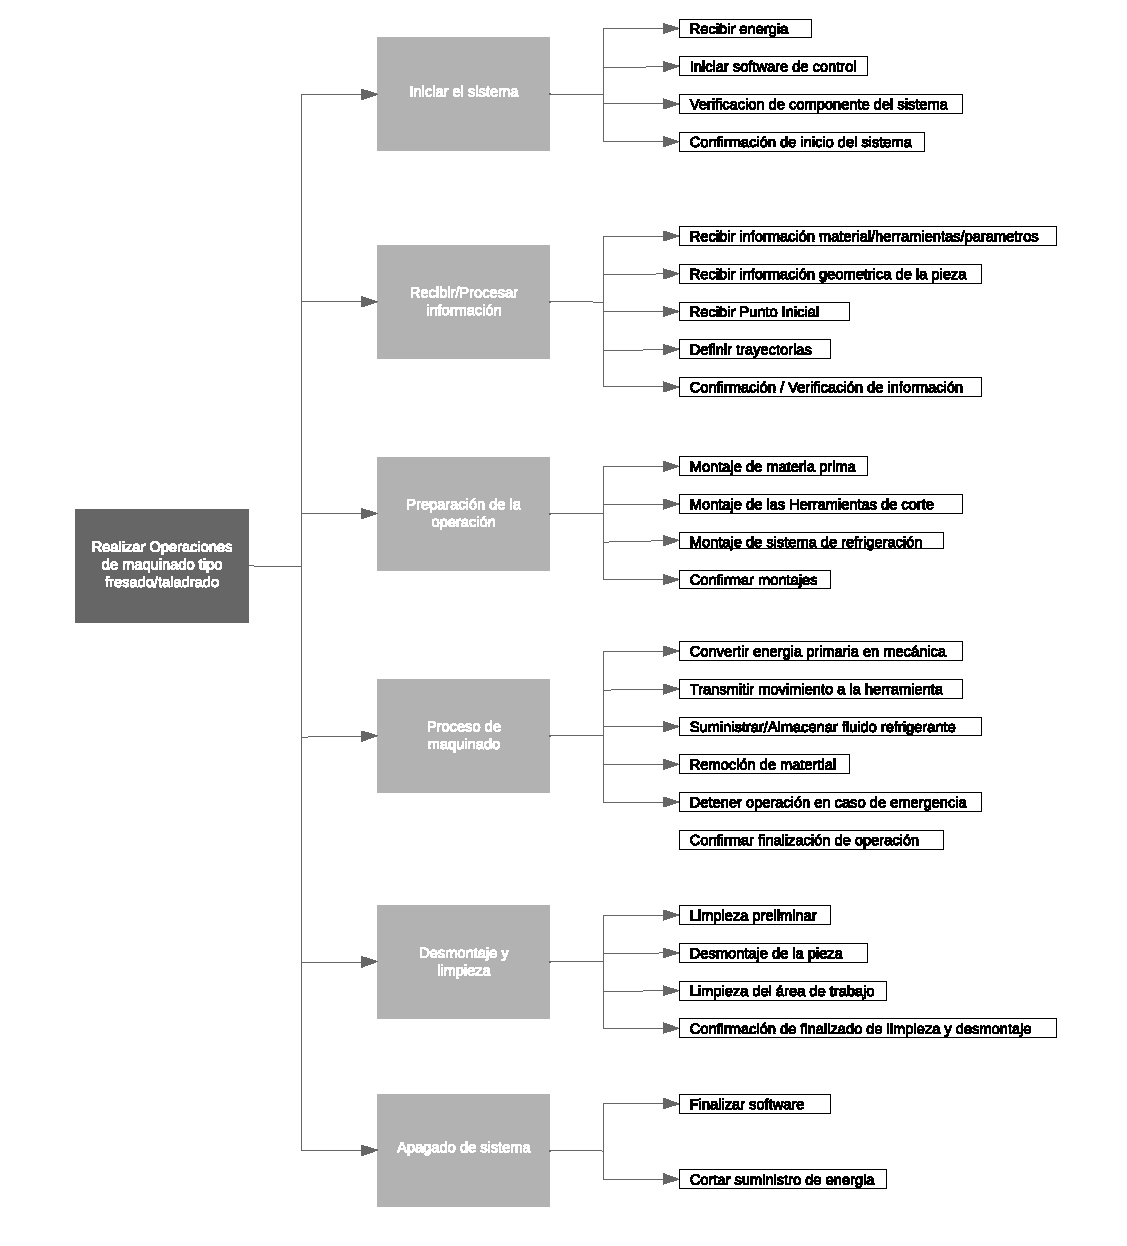
\includegraphics[width = \textwidth]{Cap3_DisenoConceptual/Figura/DespliegueFuncional.pdf}
    \caption{Despliegue de Funciones de la Máquina Herramienta}{Fuente: Elaboración Propia}
    \label{fig:DespliegueFuncional}
\end{figure}

\subsubsection{Descripción detallada de las funciones}
El buen funcionamiento de la máquina herramienta se lleva a cabo a través de las funciones presentadas a continuación:

\textbf{Iniciar el sistema}: Es necesario suministrar energía eléctrica a la máquina, de esta manera encender el sistema de control que esta posee. Al iniciar este proceso se verifican los componentes de la máquina y se recibe una confirmación por parte del sistema de control indicando que la máquina se encuentra lista para empezar a ser configurada para la operación. 

\textbf{Recibir/Procesar información}: El técnico encargado de la operación de maquinado se encargará de suministrar la información sobre el material, herramientas de corte y parámetros de la operación. así mismo el técnico suministra lo geometría de la pieza de trabajo (geometría inicial y final). Es necesario que antes de la operación tener un punto cero de referencia. Teniendo ya los datos anteriores el software definirá las trayectorias y velocidades a las que se realizarán los cortes. El software confirmara que todos los parámetros estén bien definidos y mostrará un resumen de operación para que el técnico de pueda dar inicio a la operación.

\textbf{Preparar operación de maquinado}: Una vez el operario haya iniciado el sistema procederá a realizar el montaje de la materia prima con la que se realizará el trabajo, así como el montaje de la herramienta de corte idónea para los resultados y/o requerimientos finales de la pieza a fabricar.  En estos procesos de maquinado donde el desbaste de material genera una cantidad de calor considerable resulta importante contar con un sistema de refrigeración el cual será montado por el operario. Para finalizar y garantizar el buen funcionamiento el operario debe confirmar los montajes realizados.

\textbf{Iniciar proceso de maquinado}:  Una vez finalizadas las funciones previas, la máquina debe transformar la energía eléctrica a energía mecánica para comenzar con el movimiento de los elementos de la máquina. Partiendo del movimiento de los actuadores se debe transmitir el movimiento a la herramienta, teniendo en cuenta las potencias requeridas. En este punto la máquina-herramienta se encuentra lista para empezar con la remoción de material. Hasta el final del proceso de remoción de material la máquina debe suministrar fluido de refrigeración a la zona en herramienta pieza que se encuentran en operación. En caso de alguna emergencia o mal funcionamiento se debe poder detener la operación. Si todo el procedimiento se lleva a cabo de manera adecuada se recibirá una confirmación de finalización de la operación. 

\textbf{Desmontar y limpiar pieza y área de trabajo}: Después de que la operación de maquinado haya finalizado, la máquina comenzará una limpieza preliminar con un chorro de aire para retirar la viruta de la superficie de la pieza maquinada. Después el técnico encargado retirar la pieza de trabajo y dar inicio a la limpieza del área de trabajo.

\textbf{Apagar de sistema}: Una vez finalizado todo es proceso de mecanizado y limpieza, sabiendo que no se hará otra operación de maquinado el técnico que opera la máquina apagará el software y quitará el fluido eléctrico de la máquina.

%%%%%   Análisis Funcional    %%%%%
\subsection{Análisis Funcional}
\label{sec:AnalisisFuncional}

El análisis funcional busca producir un diagrama de bloques, que represente los flujos de energía, material, y señal (o información) como flechas etiquetadas tomando un camino entre los bloques de funciones. El análisis funcional más general consta de un simple bloque de función, la cual describe la función global del dispositivo; este diagrama se conoce como \enquote{caja negra} y es un punto de partida pare el diseño de nuevos equipos o dispositivos. Luego de esto, y con ayuda de lo encontrado en el despliegue de funciones, es posible generar un diagrama que interrelacione todas las subfunciones del producto, así como los flujos que conectan a estas; este nuevo diagrama se le conoce como \enquote{Caja transparente} \citep{dieter2012engineering}.

Los diagramas obtenidos para este proyecto se pueden observar en las figuras \ref{fig:CajaNegra} y \ref{fig:CajaTransparente}.

\begin{figure}[htb!]
    \centering
    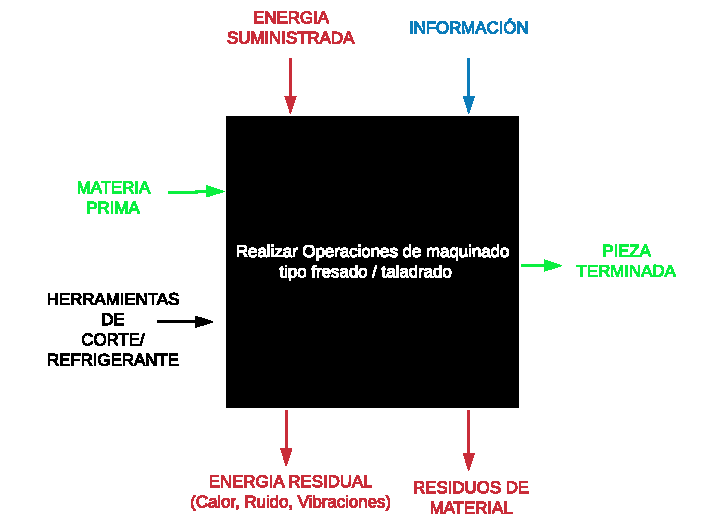
\includegraphics[width =  \textwidth]{Cap3_DisenoConceptual/Figura/CajaNegra.pdf}
    \caption{Caja Negra de la Máquina Herramienta}{Fuente: Elaboración Propia}
    \label{fig:CajaNegra}
\end{figure}

\begin{figure}[htb!]
    \centering
    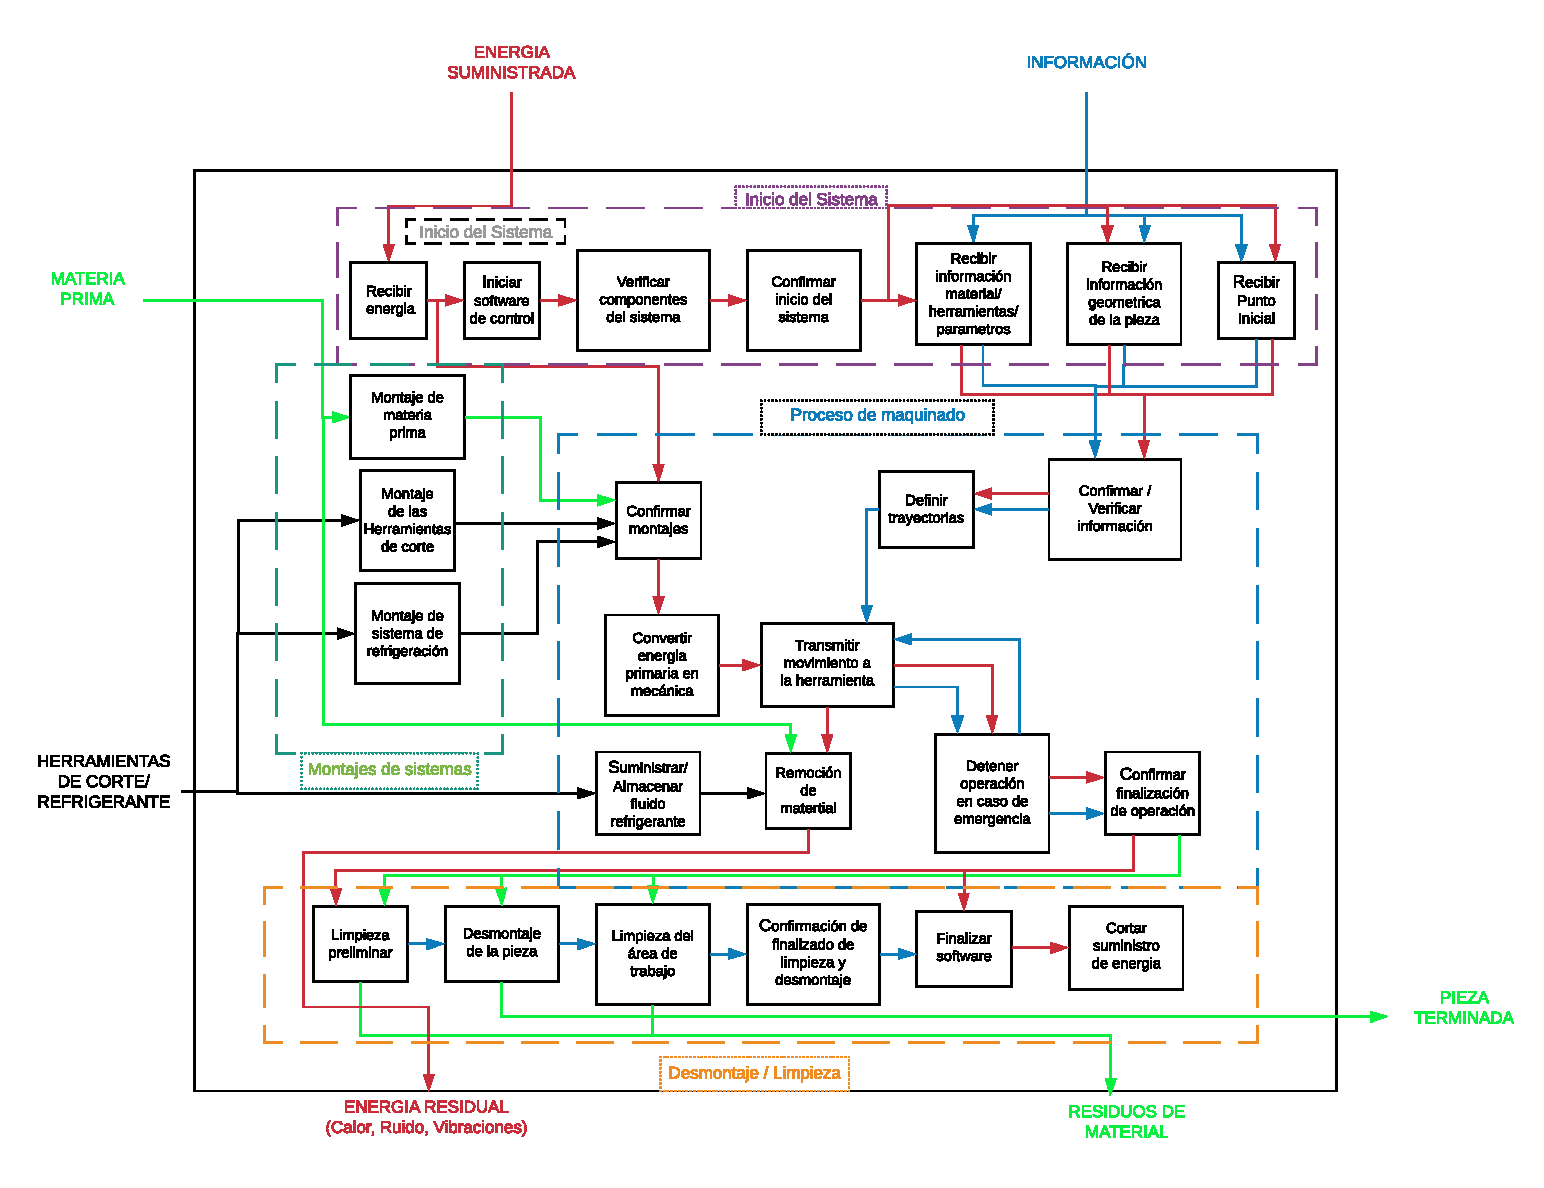
\includegraphics[width= \textwidth]{Cap3_DisenoConceptual/Figura/CajaTransparente.pdf}
    \caption{Caja Transparente de la Máquina Herramienta}{Fuente: Elaboración Propia}
    \label{fig:CajaTransparente}
\end{figure}

\newpage

%%%%%   Definición y ponderación de criterios de selección    %%%%%
\section{Definición y ponderación de criterios de selección}
Las alternativas de diseño de conceptuales que se sean planteadas deben satisfacer unos criterios para ser seleccionada como mejor alternativa. Estos criterios, aparte de las especificaciones de diseño, son indicadores del nivel de rendimiento de la solución, de ahí que se implemente un método sistemático cuantitativo para la evaluación de las alternativas. Para este proyecto se harán uso de nueve criterios que diseño, que compren factores económicos, rendimiento mecánico, diseño amigable con el medio ambiente y seguridad.

\subsection{Descripción detallada de las criterios de selección}
\textbf{Costo de Adquisición}: Es altamente deseable un bajo costo de adquisición para la maquina puesto que el mercado objetivo son las Pymes y la solución brindada debe estar asequible.

\textbf{Costo de Mantenimiento}: Se requiere que sea mínimo para reducir costos operativos y de producción, se relaciona con el número de piezas, modularidad y estandarización de las piezas de la máquina.

\textbf{Costo operativo/ Operación Ecológica}: Se requiere que sean bajos ya que te permite estimar la minimización de los costos del producto final.

\textbf{Precisión/Rigidez}: Se requiere una alta precisión y rigidez en la maquina herramienta debido a que se producirán piezas con bajas tolerancias y de alta calidad que logren ser competitivas en un mercado internacional.

\textbf{Seguridad}: Es altamente deseado, ya que permite que durante el proceso de producción tanto la pieza como el operador sufra una pérdida significativa.

\textbf{Compacidad}: Se desea una relación de compacidad alta donde la maquina pueda optimizar el espacio disponible en campo y conservar un espacio de trabajo para poder trabajar con piezas de mayor tamaño.

\textbf{Re configurabilidad}: El modularidad hace referencia a la posibilidad de hacer módulos (sistemas interconectables e intercambiables) de manera tal que facilite la posibilidad de hacer modificaciones de módulos en particular, ya sea para mejora de un módulo o para cambiar la función de este.

\textbf{Control}: Es altamente deseado, este disminuye el tiempo operativo, aumenta la precisión, minimiza las vibraciones, y aumenta la capacidad de operación hace referencia al control tanto de la máquina operativa como control en los factores externos.

\textbf{Capacidad de Carga}: Es altamente deseada para aumentar la productividad, poder maquinar materiales más resistentes, manejar mayores velocidades de maquinado y mayor durabilidad de los componentes de la máquina.

\subsection{Matriz de comparación de los criterios de selección}
\begin{landscape}
    \begin{table}
\centering
\footnotesize
\begin{tabular}{|>{\columncolor[gray]{0.85}}c|c|c|c|c|c|c|c|c|c|c|c|c|c|c|c|c|c|c|c|}
\rowcolor[gray]{0.85} \hline
\multicolumn{19}{|c|}{Matriz de comparacion por pares - CRITERIOS}\\ \hline
\rowcolor[gray]{0.85}
\textbf{Criterios} & \rotatebox{90}{Costo de Adquisicion} & \rotatebox{90}{Costo de Mantenimiento} & \rotatebox{90}{Costo operativo} & \rotatebox{90}{Precision / Rigidez} & \rotatebox{90}{Seguridad} & \rotatebox{90}{Compacidad} & \rotatebox{90}{Reconfigurabilidad} & \rotatebox{90}{Control} & \rotatebox{90}{Capacidad de Carga} & \multicolumn{9}{c|}{Matriz Normalizada}\\ \hline
Costo de Adquisicion    & 1  & 5 & 5   & 1/5 & 1/3 & 9 & 5 & 3   & 5   & 0,10 & 0,17 & 0,24 & 0,06 & 0,09 & 0,15 & 0,13 & 0,33 & 0,22\\ \hline
Costo de Mantenimiento  & 1/5& 1 & 1/3 & 1/7 & 1/5 & 5 & 1 & 1/5 & 1/3 & 0,02 & 0,03 & 0,02 & 0,04 & 0,05 & 0,08 & 0,03 & 0,02 & 0,01\\ \hline
Costo operativo         & 1/5& 3 & 1   & 1/5 & 1/5 & 8 & 6 & 1/3 & 1   & 0,02 & 0,10 & 0,05 & 0,06 & 0,05 & 0,14 & 0,15 & 0,04 & 0,04\\ \hline
Precision / Rigidez     & 5  & 7 & 5   & 1   & 1   & 9 & 7 & 2   & 5   & 0,49 & 0,23 & 0,24 & 0,29 & 0,27 & 0,15 & 0,18 & 0,22 & 0,22\\ \hline
Seguridad               & 3  & 5 & 5   & 1   & 1   & 9 & 7 & 2   & 5   & 0,29 & 0,17 & 0,24 & 0,29 & 0,27 & 0,15 & 0,18 & 0,22 & 0,22\\ \hline
Compacidad              & 1/9&1/5& 1/8 & 1/9 & 1/9 & 1 &1/4& 1/9 & 1/5 & 0,01 & 0,01 & 0,01 & 0,03 & 0,03 & 0,02 & 0,01 & 0,01 & 0,01\\ \hline
Reconfigurabilidad      & 1/5& 1 & 1/6 & 1/7 & 1/7 & 4 & 1 & 1/7 & 1/5 & 0,02 & 0,03 & 0,01 & 0,04 & 0,04 & 0,07 & 0,03 & 0,02 & 0,01\\ \hline
Control                 & 1/3& 5 & 3   & 1/2 & 1/2 & 9 & 7 & 1   & 5   & 0,03 & 0,17 & 0,15 & 0,14 & 0,14 & 0,15 & 0,18 & 0,11 & 0,22\\ \hline
Capacidad de Carga      & 1/5& 3 & 1   & 1/5 & 1/5 & 5 & 5 & 1/5 & 1   & 0,02 & 0,10 & 0,05 & 0,06 & 0,05 & 0,08 & 0,13 & 0,02 & 0,04\\ \hline
\textbf{Total}          & 10,24 & 30,20 & 20,63 & 3,50 & 3,69 & 9,00  &39,25 & 8,99 & 22,73\\ \cline{1-10}
\textbf{Promedio}       & 16,52 & 3,46 & 7,20 & 25,48 & 22,57 & 1,44 & 2,87 & 14,27 & 6,19\\ \cline{1-14}
\textbf{AxP}            & 1,84 & 0,32 & 0,70 & 2,83 & 2,43 & 0,14 & 0,27 & 1,47 & 0,61 & $ {\overline{\lambda}} $  & CI & RI & CR \\ \cline{1-14}
${\lambda}$             & 11,11 & 9,35 & 9,75 & 11,13 & 10,79 & 9,53 & 9,32 & 10,28 & 9,87 & 10,12 & 0,14 & 1,45 & 0,09 \\ \cline{1-14}

\end{tabular}
\caption{Matriz de comparación de los criterios de selección}{Fuente: Elaboración Propia}
\label{table:pairMatrix}
\end{table}
\end{landscape}

%%%%%   Selección de la tecnología de Máquina Herramienta    %%%%%
\section{Selección de la tecnología de Robot Herramienta}
\ref{section:DefiniciondeEspeficaciones}
A partir de lo encontrado en la definición de especificaciones (ver Capitulo \ref{section:DefiniciondeEspeficaciones}), fueron encontradas 3 tecnologías de mecanismos empleados como máquinas herramientas, estos son las máquinas convencionales (con sistema cartesiano), robots seriales (con lazo abierto) y manipuladores paralelos (lazo cerrado). Cada uno con sus ventajas y desventajas, por lo que para una buena generación de alternativas se comparó el rendimiento de estas tecnologías según los criterios de selección y determinar cuál es la mejor tecnología para esta aplicación. Se empleó un método de asignación directa para la evaluación, y las ponderaciones se basan de lo visto en la literatura. A parte de esto, se realiza un análisis de robustez de la solución, donde se concluye que las opciones convencionales y paralelas son las mejores para este proyecto.

\begin{longtable}{|>{\columncolor[gray]{0.85}} p{0.25\textwidth}| c | c   c   c |}
    \hline \rowcolor[gray]{0.85}
     & \rotatebox{90}{\textbf{Importancia}} & \rotatebox{90}{\textbf{Convencional~}} & \rotatebox{90}{\textbf{Serial}} & \rotatebox{90}{\textbf{Paralela}} \\ \hline \endhead
    Costo de Adquisición & 20 & 10 &  5 &  7\\ \hline
    Costo Mantenimiento  & 10 &  9 &  7 &  5\\ \hline
    Precision/Rigidez    & 20 &  8 &  5 & 10\\ \hline
    Seguridad            &  5 &  8 &  7 &  9\\ \hline
    Compacidad           &  5 &  6 & 10 &  7\\ \hline
    Modularidad          & 10 &  7 &  7 & 10\\ \hline
    Control              &  5 & 10 &  8 &  6\\ \hline
    Capacidad de carga   & 15 &  7 &  5 &  9\\ \hline
     & 100 & \textbf{36.38} & 26.34 & \textbf{37.28} \\ \hline
    \caption{Selección de Tecnología }{Fuente: Elaboración Propia}
    \label{table:SeleccionTecnologia}
\end{longtable}

\section{Análisis morfológico}

Con el objetivo de conformar diversas alternativas, se decidió realizar un análisis morfológico el cual permitiera identificar posibles soluciones que cumpliesen las subfunciones planteadas anteriormente en el despliegue de funciones. En este análisis se evaluaron 3 posibles soluciones para cada subfunción y se plasmo el conjunto en una tabla.
\small
\begin{longtable}{| >{\columncolor[gray]{0.85}} c | >{\columncolor[gray]{0.85}} c | >{\columncolor[gray]{0.85}} p{0.2\textwidth} | p{0.15\textwidth}   p{0.15\textwidth}   p{0.15\textwidth} |}

\hline \rowcolor[gray]{0.85}
 Función & N & Subfunción                               & Concepto de solución 1      & Concepto de solución 2   & Concepto de solución 3 \\ \hline \endhead
 & 1 & Tipo de alimentación de energía          & Electrica                     & Hidraulica & Neumatica \\ \cline{2-6}
 & 2 & Transmitir energía hacia los componentes & Conexiones eléctrica        & Tuberia hidraulica  & Tuberia Neumatica \\ \cline{2-6}
 & 3 & Sistema de control                       & Computarizado               & Manual                   & Semiautomático\\ \cline{2-6}
\multirow{-4}{*}{ Iniciar Sistema}& 4 & Software                                 & Arduino                     & Python                   & LabVIEW\\ \hline
 
 &  5 & Montaje de herramienta de corte          & Acople magnético            & Acople tipo mordaza      &\\  \cline{2-6}
 &  6 & Sujeción de materia prima                & Mordazas mecánicas          & Mordazas hidráulicas       & Mordazas neumáticas  \\ \cline{2-6}
\multirow{-3}{*}{Preparar Montajes} &  7 & Sistema de refrigeración                 & Refrigeración por aire      & Refrigeración por liquido & Refrigeración Mixto\\ \cline{1-6}
 &  8 & Cinemática                               & Convencional                & Paralela (Try-Piramid)    & Paralela (UPU)\\ \cline{2-6}

 & 9 & Actuadores                               & Motor paso a paso           & Motores síncronos	       & \\ \cline{2-6}
 & 10 & Sistema de guiado                        & Rieles                      & Ejes                     & Cable\\ \cline{2-6}

 
 & 11 & Sistema de transmisión de movimiento     & Tornillo de potencia        & Cilindro-pistón           & Transmisión por correa\\ \cline{2-6}
 \multirow{-4}{*}{ Mecanizar} & 12 & Sistema de parada de emergencia          & Sistema mecánico bloqueante & Sistema corta corriente   & \\ \hline

 & 13 & Sistema de limpieza                      & Aire comprimido             & Agua a presión            & Barrido manual\\ \cline{2-6}
  \multirow{-2}{*}{ Finalizar operación} & 14 & Confirmar finalización de operación      & Indicador led               & Indicador digital         & Indicador sonoro \\ \hline

\caption{Diagrama Morfológico}
\label{table:DiagramaMorfologico}
\end{longtable}

\newpage
\section{Generación de Alternativas}

\subsection{Alternativa 1: Máquina Herramienta Convencional}

\subsubsection{Resumen de la alternativa} La principal característica que presenta la alternativa 1 es la estructura tipo cartesiana que brinda 3 grados de libertad conforme a los ejes cartesianos. En este caso, el mecanismo de la maquina es movido por 3 motores paso a paso ubicados en cada eje, los cuales mueven un carro mediante un tornillo de potencia. El movimiento de cada carro es guiado por un sistema de rieles ubicados de forma tal que permitan alcanzar el espacio de trabajo deseado. El mecanismo consta de un motor ubicado en el eje z (Vertical) que es el encargado de mover la herramienta de corte.
En el carro correspondiente al eje Y, se dispone un sistema de guiado en el cual se montan unas mordazas mecánicas las cuales son las encargadas de sujetar el material a mecanizar.
Por otra parte, el proceso de mecanizado será llevado a cabo por un proceso de control numérico computarizado, específicamente con el interfaz de Python.

\subsubsection{Descripción}
Con base al análisis morfológico y la síntesis funcional, se selecciono los conceptos para el funcionamiento de la alterativa 1, generando el siguiente diagrama morfológico de la alternativa. 
\input{Cap3_DisenoConceptual/Tablas/Solución1.tex}

\begin{figure}[htb!]
    \centering
    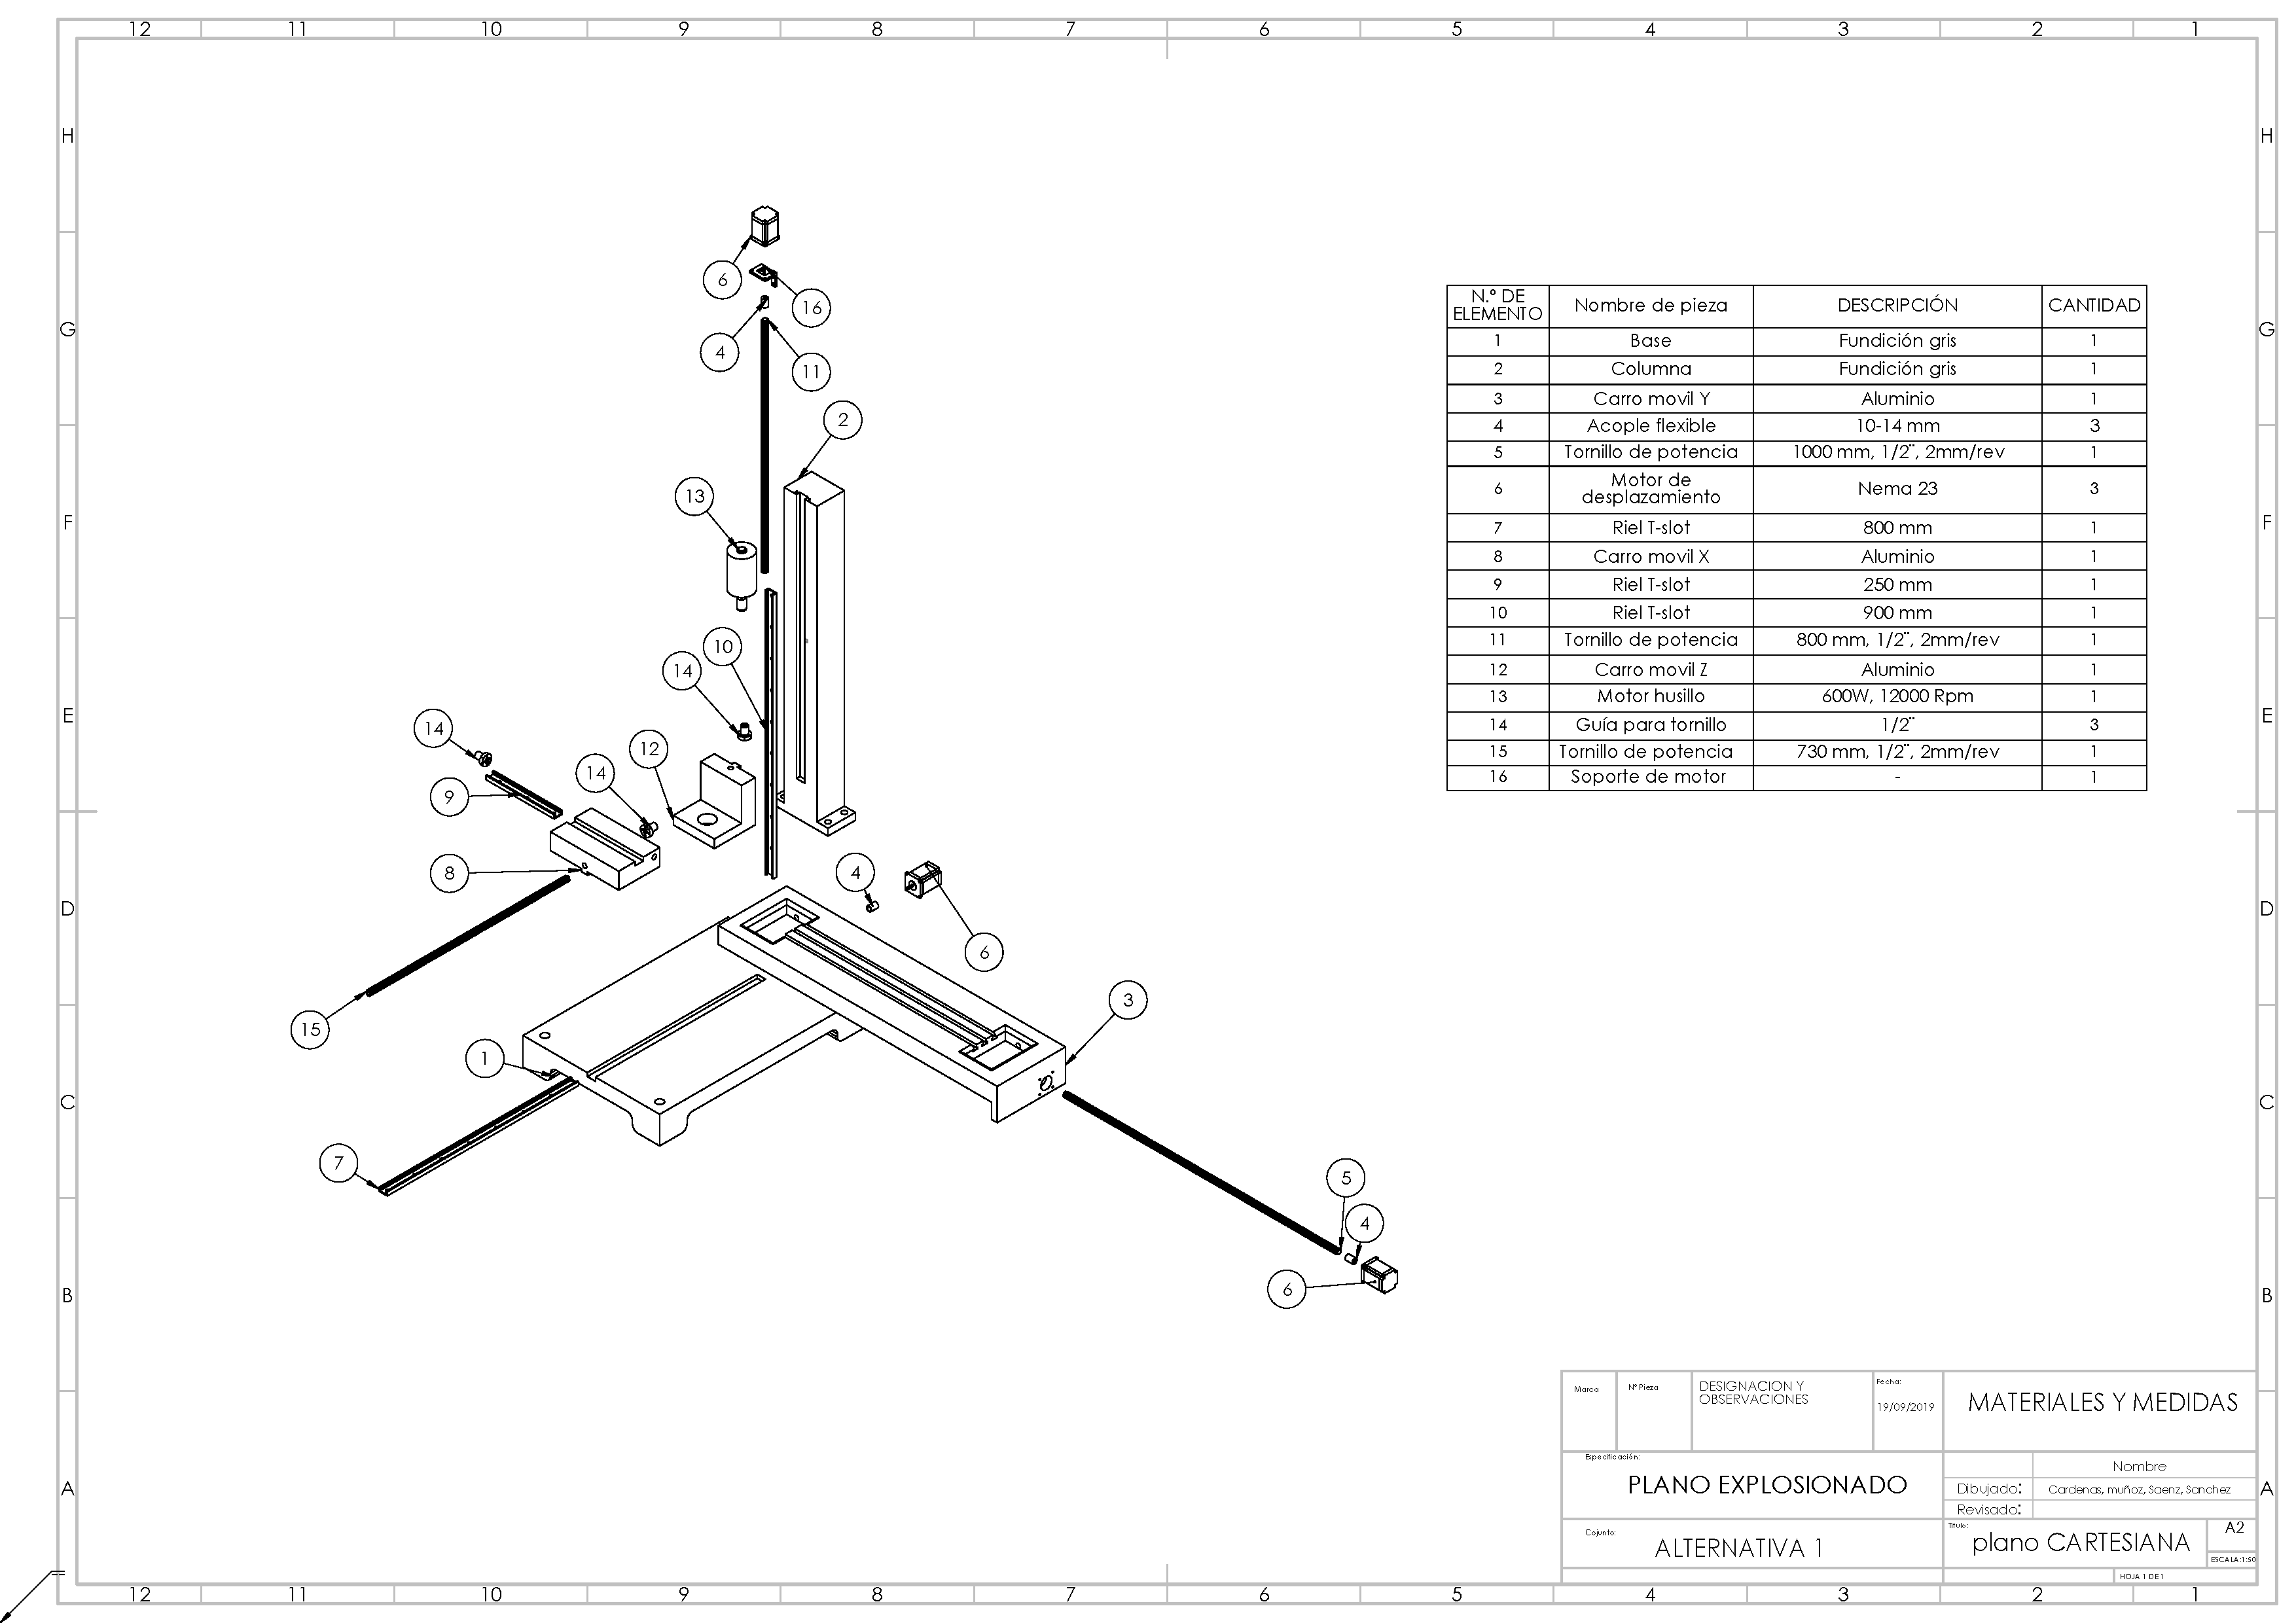
\includegraphics[width =  \textwidth]{Cap3_DisenoConceptual/Figura/Plano_alt_1.pdf}
    \caption{Plano Explosionado y lista de materiales de la alternativa 1}{Fuente: Elaboración Propia}
    \label{fig:Plano_alt_1}
\end{figure}

\subsubsection{Presupuesto}
Una vez con el concepto de la alternativa establecido, se procedió a realizar un presupuesto, el cuál tenga en cuenta las diferentes fases de vida de la alternativa, es decir desde el diseño hasta la fabricación para la posterior evaluación de viabilidad de la alternativa.
\begin{longtable}{| c | p{0.32\textwidth} | r | r | c | r |}
\hline \rowcolor[gray]{0.85}
 & Descripción & \multicolumn{1}{c|}{Valor Unitario} & \multicolumn{1}{c|}{Cantidad} & Unidades & \multicolumn{1}{c|}{Valor}  \\ \hline \endhead
\multirow{5}{*}{\rotatebox{90}{Diseño}}
 & Ingeniero de calculo	& \$ 150.000,00 & 40,00 & horas & \$ 6.000.000,00\\
 & Memorias y plano & \$ 15.000,00 & 80,00	& horas	& \$ 1.200.000,00 \\
 & Software & \$ 500.000,00 &	1,00 &	-	& \$ 500.000,00 \\
 & Interfaz	& \$ 500.000,00 &	1,00 &	-	& \$ 500.000,00 \\
\cline{2-6} & \multicolumn{4}{c|}{ \textbf{Subtotal Diseño}} & \$ \textbf{8.200.000,00}  \\ \hline

% \multirow{18}{*}{\rotatebox{90}{Lista de Componentes}}
 & Motor Paso a Paso Nema 23 28.55 Kg.cm	 & \$ 225.676,00 & 3,00 & -	 & \$ 677.028,00 \\
 & Motor-Husillo 600W max,48 V max, 1200 Rpm max, DC	 & \$ 400.000,00 & 1,00 & -	 & \$ 400.000,00 \\
 & Tornillo de potencia 12 mm	 & \$ 45.000,00 & 3,00 & -	 & \$ 135.000,00 \\
 & Acople Flexible D30L42 10X14 mm	 & \$ 35.890,00 & 3,00 & -	 & \$ 107.670,00 \\
 & Riel T slot	 & \$ 75.000,00 & 3,00 & -	 & \$ 225.000,00 \\
 & Guia para tornillo 	 & \$ 120.000,00 & 3,00 & -	 & \$ 360.000,00 \\
 & Columna 	 & \$ 5.000,00 & 87,00 & Kg	 & \$ 435.000,00 \\
 & Base  	 & \$ 5.000,00 & 155,00 & -	 & \$ 775.000,00 \\
 & Driver motor paso a paso Nema 23	 & \$ 65.000,00 & 3,00 & -	 & \$ 195.000,00 \\
 & Carro movil eje Z	 & \$ 15.000,00 & 4,00 & Kg	 & \$ 60.000,00 \\
 & Carro movil eje Y	 & \$ 15.000,00 & 39,00 & Kg	 & \$ 585.000,00 \\
 & Carro movil eje X	 & \$ 4.000,00 & 6,00 & Kg	 & \$ 24.000,00 \\
 & Ordenador PC	 & \$ 3.600.000,00 & 1,00 & -	 & \$ 3.600.000,00 \\
 & Accesorios electricos	 & \$ 300.000,00 & 1,00 & -	 & \$ 300.000,00 \\
 & Tornilleria 	 & \$ 300.000,00 & 1,00 & -	 & \$ 300.000,00 \\
 & Sistema de limpieza	 & \$ 400.000,00 & 1,00 & -	 & \$ 400.000,00 \\
 & Sistema de refrigeración	 & \$ 600.000,00 & 1,00 & -	 & \$ 600.000,00 \\
 & Sistema de sujeccion	 & \$ 500.000,00 & 1,00 & - & \$ 500.000,00 \\
\cline{2-6}
\multirow{-18}{*}{\rotatebox{90}{Lista de Componentes}} & \multicolumn{4}{c|}{\textbf{Subtotal Lista de Componentes}} & \$ \textbf{9.678.698,00} \\ \hline

\multirow{4}{*}{\rotatebox{90}{Fabricación}}
 & Emsablador	 & \$ 10.000,00 & 24,00 & horas	 & \$ 240.000,00 \\
 & Ayudante 	 & \$ 6.000,00 & 24,00 & horas	 & \$ 144.000,00 \\
 & Surpervisor	 & \$ 100.000,00 & 8,00 & horas	 & \$ 800.000,00 \\
 \cline{2-6} & \multicolumn{4}{c|}{\textbf{Subtotal Fabricación}} & \$ \textbf{1.184.000,00} \\ \hline

\multirow{4}{*}{\rotatebox{90}{Equipos}} 
 & Pintura 	 & \$ 20.000,00 & 4,00 & m2 & \$ 80.000,00 \\
 & Herramientas	 & \$ 350.000,00 & 1,00 & - & \$ 350.000,00 \\
 & Centro de mecanizado & \$ 90.000,00 & 16,00 & horas & \$ 1.440.000,00 \\
 \cline{2-6} & \multicolumn{4}{c|}{\textbf{Subtotal Sección}} & \$ \textbf{1.870.000,00} \\ \hline

\rowcolor[gray]{0.85} \multicolumn{5}{|c|}{\textbf{Subtotal}} & \$ \textbf{20.932.698,00} \\ \hline
\multicolumn{5}{|c|}{\textbf{Imprevistos (30\%)}} & \$ \textbf{6.279.809,40} \\ \hline
\rowcolor[gray]{0.85} \multicolumn{5}{|c|}{\textbf{Total}} & \$ \textbf{27.212.507,40} \\ \hline
\caption{Presupuesto de la Alternativa 1}{Fuente: Elaboración Propia}
\end{longtable}


\subsection{Alternativa 2: Máquina Herramienta Ponchohedron}
\subsubsection{Resumen de la alternativa} 
La principal característica que presenta la alternativa 2 es su inspiración en lo encontrado en el trabajo de \cite{ZENG2014648}, en donde se presenta una familia de mecanismos del estilo Try-Pyramid. El robot escogido para la solución consta de una base triangular, en donde los bordes de esta son las prismáticas de las entradas. Los carros están conectados a la plataforma por medio de una paralelogramo formado por dos brazos y juntas universales. Por la plataforma, la cual posee una forma hexagonal que permiten conectar los tres paralelogramos. Esto generando tres grados de libertad lineales, lo que implica utilizar tres entradas, y que para este mecanismo deben ser lineales. Para esto, se utiliza la combinación de motor paso a paso acoplado a un eje roscado.
La sujeción de la pieza a la máquina se realiza por medio de un sistema neumático que estará soportado en una estructura aparte.
Por otra parte, el proceso de mecanizado será llevado a cabo por un proceso de control numérico computarizado, específicamente en Arduino.

\subsubsection{Descripción }
Con base al análisis morfológico y la síntesis funcional, se selecciono los conceptos para el funcionamiento de la alterativa 2, generando el siguiente diagrama morfológico de la alternativa.
\input{Cap3_DisenoConceptual/Tablas/Solución2.tex}

\begin{figure}[htb!]
    \centering
    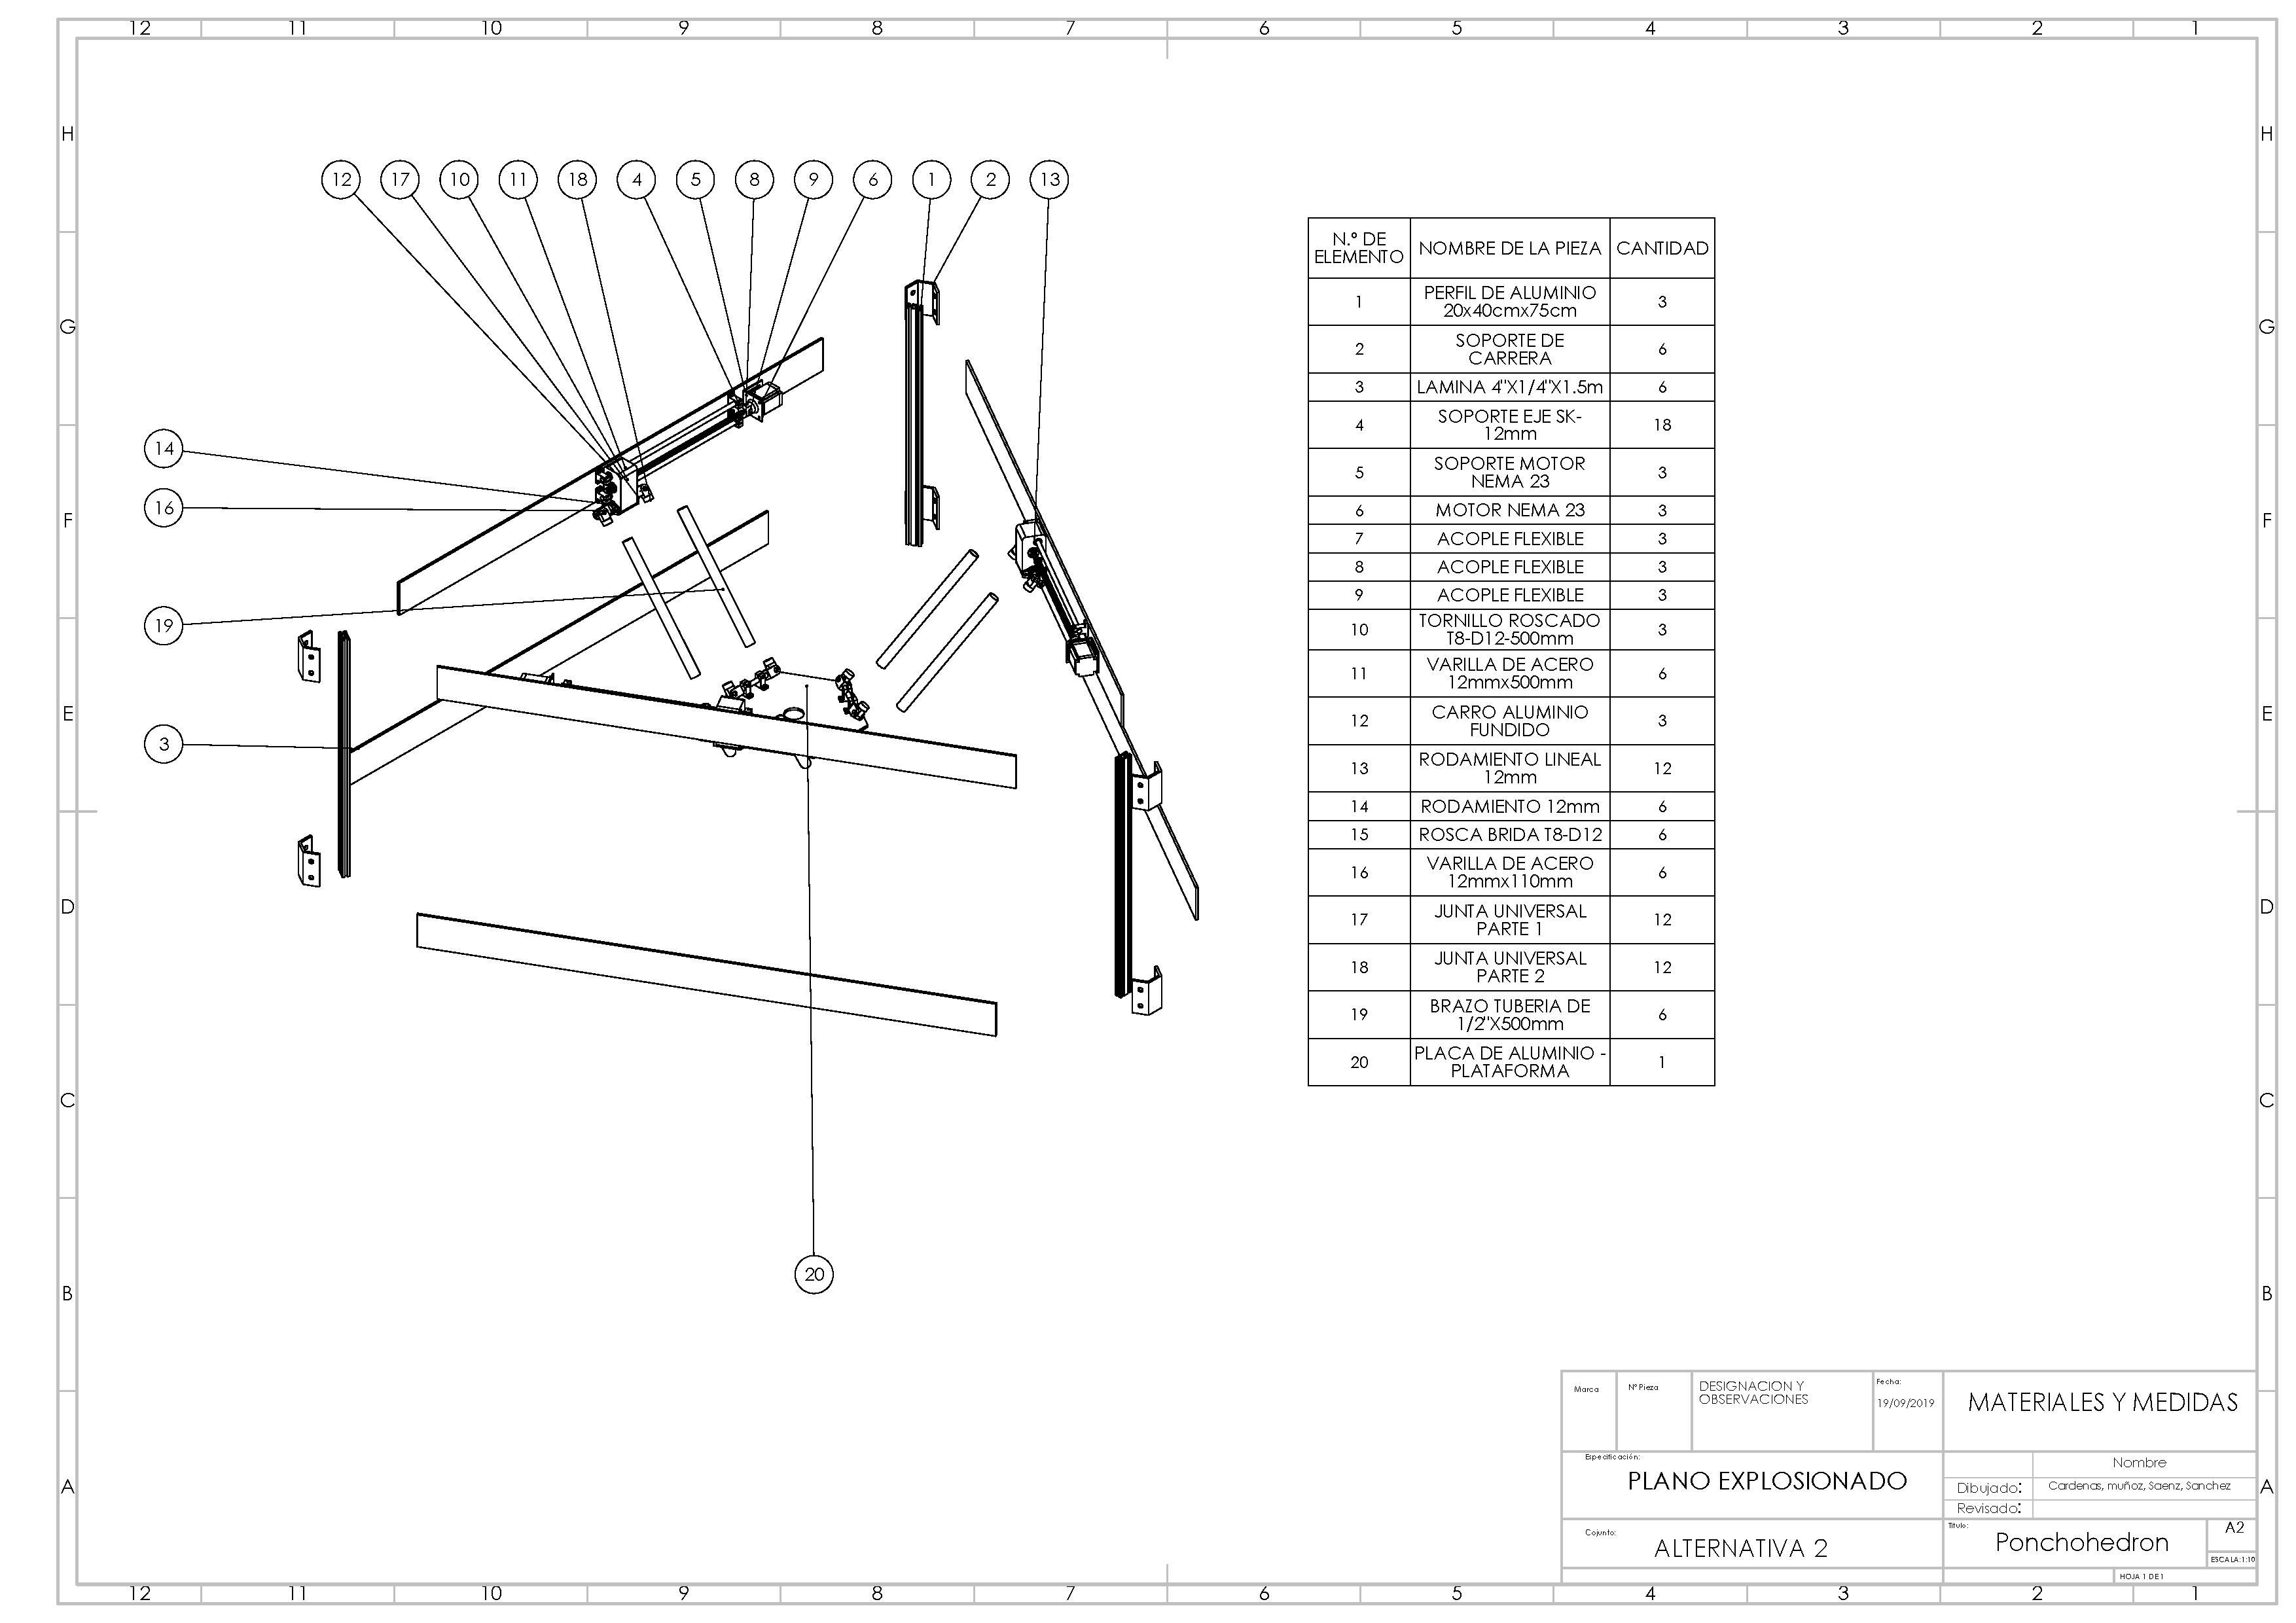
\includegraphics[width =  \textwidth]{Cap3_DisenoConceptual/Figura/Poncho.pdf}
    \caption{Plano Explosionado y lista de materiales de la alternativa 2}{Fuente: Elaboración Propia}
    \label{fig:Plano_alt_2}
\end{figure}

\newpage

\subsubsection{Presupuesto}
Una vez con el concepto de la alternativa establecido, se procedió a realizar un presupuesto para la posterior evaluación de viabilidad de la alternativa.

\begin{longtable}{| c | p{0.32\textwidth} | r | r | c | r |}
\hline \rowcolor[gray]{0.85}
 & Descripción & \multicolumn{1}{c|}{Valor Unitario} & \multicolumn{1}{c|}{Cantidad} & Unidades & \multicolumn{1}{c|}{Valor}  \\ \hline \endhead
\multirow{5}{*}{\rotatebox{90}{Diseño}}
 & Ingeniero de calculo	& \$ 150.000,00 & 60,00 & horas & \$ 9.000.000,00\\
 & Memorias y plano & \$ 15.000,00 & 40,00	& horas	& \$ 600.000,00 \\
 & Software & \$ 750.000,00 &	1,00 &	-	& \$ 750.000,00 \\
 & Interfaz	& \$ 500.000,00 &	1,00 &	-	& \$ 500.000,00 \\
\cline{2-6} & \multicolumn{4}{c|}{ \textbf{Subtotal Diseño}} & \$ \textbf{10.850.000,00}  \\ \hline

% \multirow{18}{*}{\rotatebox{90}{Lista de Componentes}}
 & Motor Paso a Paso Nema 23 28.55 Kg.cm	 & \$ 225.676,00 & 3,00 & -	 & \$ 677.028,00 \\
 & Motor-Husillo 600W max,48 V max, 1200 Rpm max, DC	 & \$ 400.000,00 & 1,00 & -	 & \$ 400.000,00 \\
 & Tornillo de potencia 12 mm	 & \$ 45.000,00 & 3,00 & -	 & \$ 135.000,00 \\
 & Acople Flexible D30L42 10 mm X 12 mm	 & \$ 40.038,91 & 3,00 & -	 & \$ 120.116,72 \\
 & Rosca Brida T8 - D 12 mm & \$ 36.904,86 & 3,00 & - & \$ 110.714,58 \\
 & Varilla de acero 12 mm x 0.5 m & \$ 34.653,00 & 6,00 & - & \$ 207.918,00 \\
 & Soporte Eje SK-12 mm & \$ 6.178,00 & 18,00 & - & \$ 111.204,00 \\
 & Lamina de aluminio de 4.5 pulg x 1/4 pulg x 1.5 m & \$ 25.000,00 & 3,00 & - & \$ 75.000,00 \\
 & Perfil de aluminio 20 mm x 40 mm x 0.75 m & \$ 72.900,00 & 3,00 & - & \$ 218.700,00 \\
 & Driver motor paso a paso Nema 23 & \$ 65.000,00 & 3,00 & - & \$ 195.000,00 \\
 & Soporte Motor NEMA 23 & \$ 16.400,00 & 3,00 & - & \$ 49.200,00 \\
 & Brazos - Tuberia 1/2 pulg x 0.5 m & \$ 30.000,00 & 6,00 & - & \$ 180.000,00 \\
 & Carro Brazos & \$ 15.000,00 & 3,30 & kg & \$ 49.500,00 \\
 & Plataforma & \$ 40.000,00 & 2,00 & kg & \$ 80.000,00 \\
 & Soporte de Carrera & \$ 24.000,00 & 6,00 & - & \$ 144.000,00 \\
 & Rodamiento Lineal LM16UU & \$ 14.875,00 & 14,00 & - & \$ 208.250,00 \\
 & Chumacera K004 FL001 & \$ 12.300,00 & 3,00 & - & \$ 36.900,00 \\
 & Ordenador PC & \$ 3.600.000,00 & 1,00 & - & \$ 3.600.000,00 \\
 & Accesorios electricos & \$ 400.000,00 & 1,00 & - & \$ 400.000,00 \\
 & Tornilleria  & \$ 200.000,00 & 1,00 & - & \$ 200.000,00 \\
 & Sistema de limpieza & \$ 500.000,00 & 1,00 & - & \$ 500.000,00 \\
 & Sistema de refrigeración & \$ 500.000,00 & 1,00 & - & \$ 500.000,00 \\
 & Sistema de sujeccion & \$ 500.000,00 & 1,00 & - & \$ 500.000,00 \\
\cline{2-6}
\multirow{-18}{*}{\rotatebox{90}{Lista de Componentes}} & \multicolumn{4}{c|}{\textbf{Subtotal Lista de Componentes}} & \$ \textbf{8.698.531,30} \\ \hline

\multirow{4}{*}{\rotatebox{90}{Fabricación}}
 & Emsablador	 & \$ 10.000,00 & 80,00 & horas	 & \$ 800.000,00 \\
 & Ayudante 	 & \$ 6.000,00 & 80,00 & horas	 & \$ 480.000,00 \\
 & Surpervisor	 & \$ 100.000,00 & 40,00 & horas	 & \$ 4.000.000,00 \\
 \cline{2-6} & \multicolumn{4}{c|}{\textbf{Subtotal Fabricación}} & \$ \textbf{5.280.000,00} \\ \hline

\multirow{4}{*}{\rotatebox{90}{Equipos}} 
 & Pintura 	 & \$ 20.000,00 & 3,00 & m2 & \$ 60.000,00 \\
 & Herramientas	 & \$ 350.000,00 & 1,00 & - & \$ 350.000,00 \\
 & Centro de mecanizado & \$ 90.000,00 & 16,00 & horas & \$ 1.440.000,00 \\
 \cline{2-6} & \multicolumn{4}{c|}{\textbf{Subtotal Sección}} & \$ \textbf{1.850.000,00} \\ \hline

\rowcolor[gray]{0.85} \multicolumn{5}{|c|}{\textbf{Subtotal}} & \$ \textbf{26.678.531,30} \\ \hline
\multicolumn{5}{|c|}{\textbf{Imprevistos (30\%)}} & \$ \textbf{8.003.559,39} \\ \hline
\rowcolor[gray]{0.85} \multicolumn{5}{|c|}{\textbf{Total}} & \$ \textbf{34.682.090,69} \\ \hline
\caption{Presupuesto de la Alternativa 2}{Fuente: Elaboración Propia}
\end{longtable}

\subsection{Alternativa 3: Máquina Herramienta RRPRR}

\subsubsection{Resumen de la alternativa}
La principal característica que presenta la alternativa 2 es su inspiración en lo encontrado en el trabajo de \cite{petko2005mechatronic}, en donde se presenta una familia de mecanismos del estilo RRPRR. El robot escogido para la solución consta de una base triangular, en donde los vértices de esto son los puntos de acople para una revolutas de giro vertical. El eslabón acoplado a esto, posee otra revoluta en su extremo opuesto pero esta gira horizontalmente. Luego de esto, está una prismática, la cual es la entrada de movimiento del sistema. Esto generando tres grados de libertad lineales, lo que implica utilizar tres entradas, y que para este mecanismo deben ser lineales. Para esto, se utiliza la combinación de motor paso a paso acoplado a un eje roscado.
La sujeción de la pieza a la máquina se realiza por medio de un sistema neumático que estará soportado en una estructura aparte.
Por otra parte, el proceso de mecanizado será llevado a cabo por un proceso de control numérico computarizado, específicamente en python.

\subsubsection{Descripción }
\input{Cap3_DisenoConceptual/Tablas/Solución3.tex}

\begin{figure}[ht!]
    \centering
    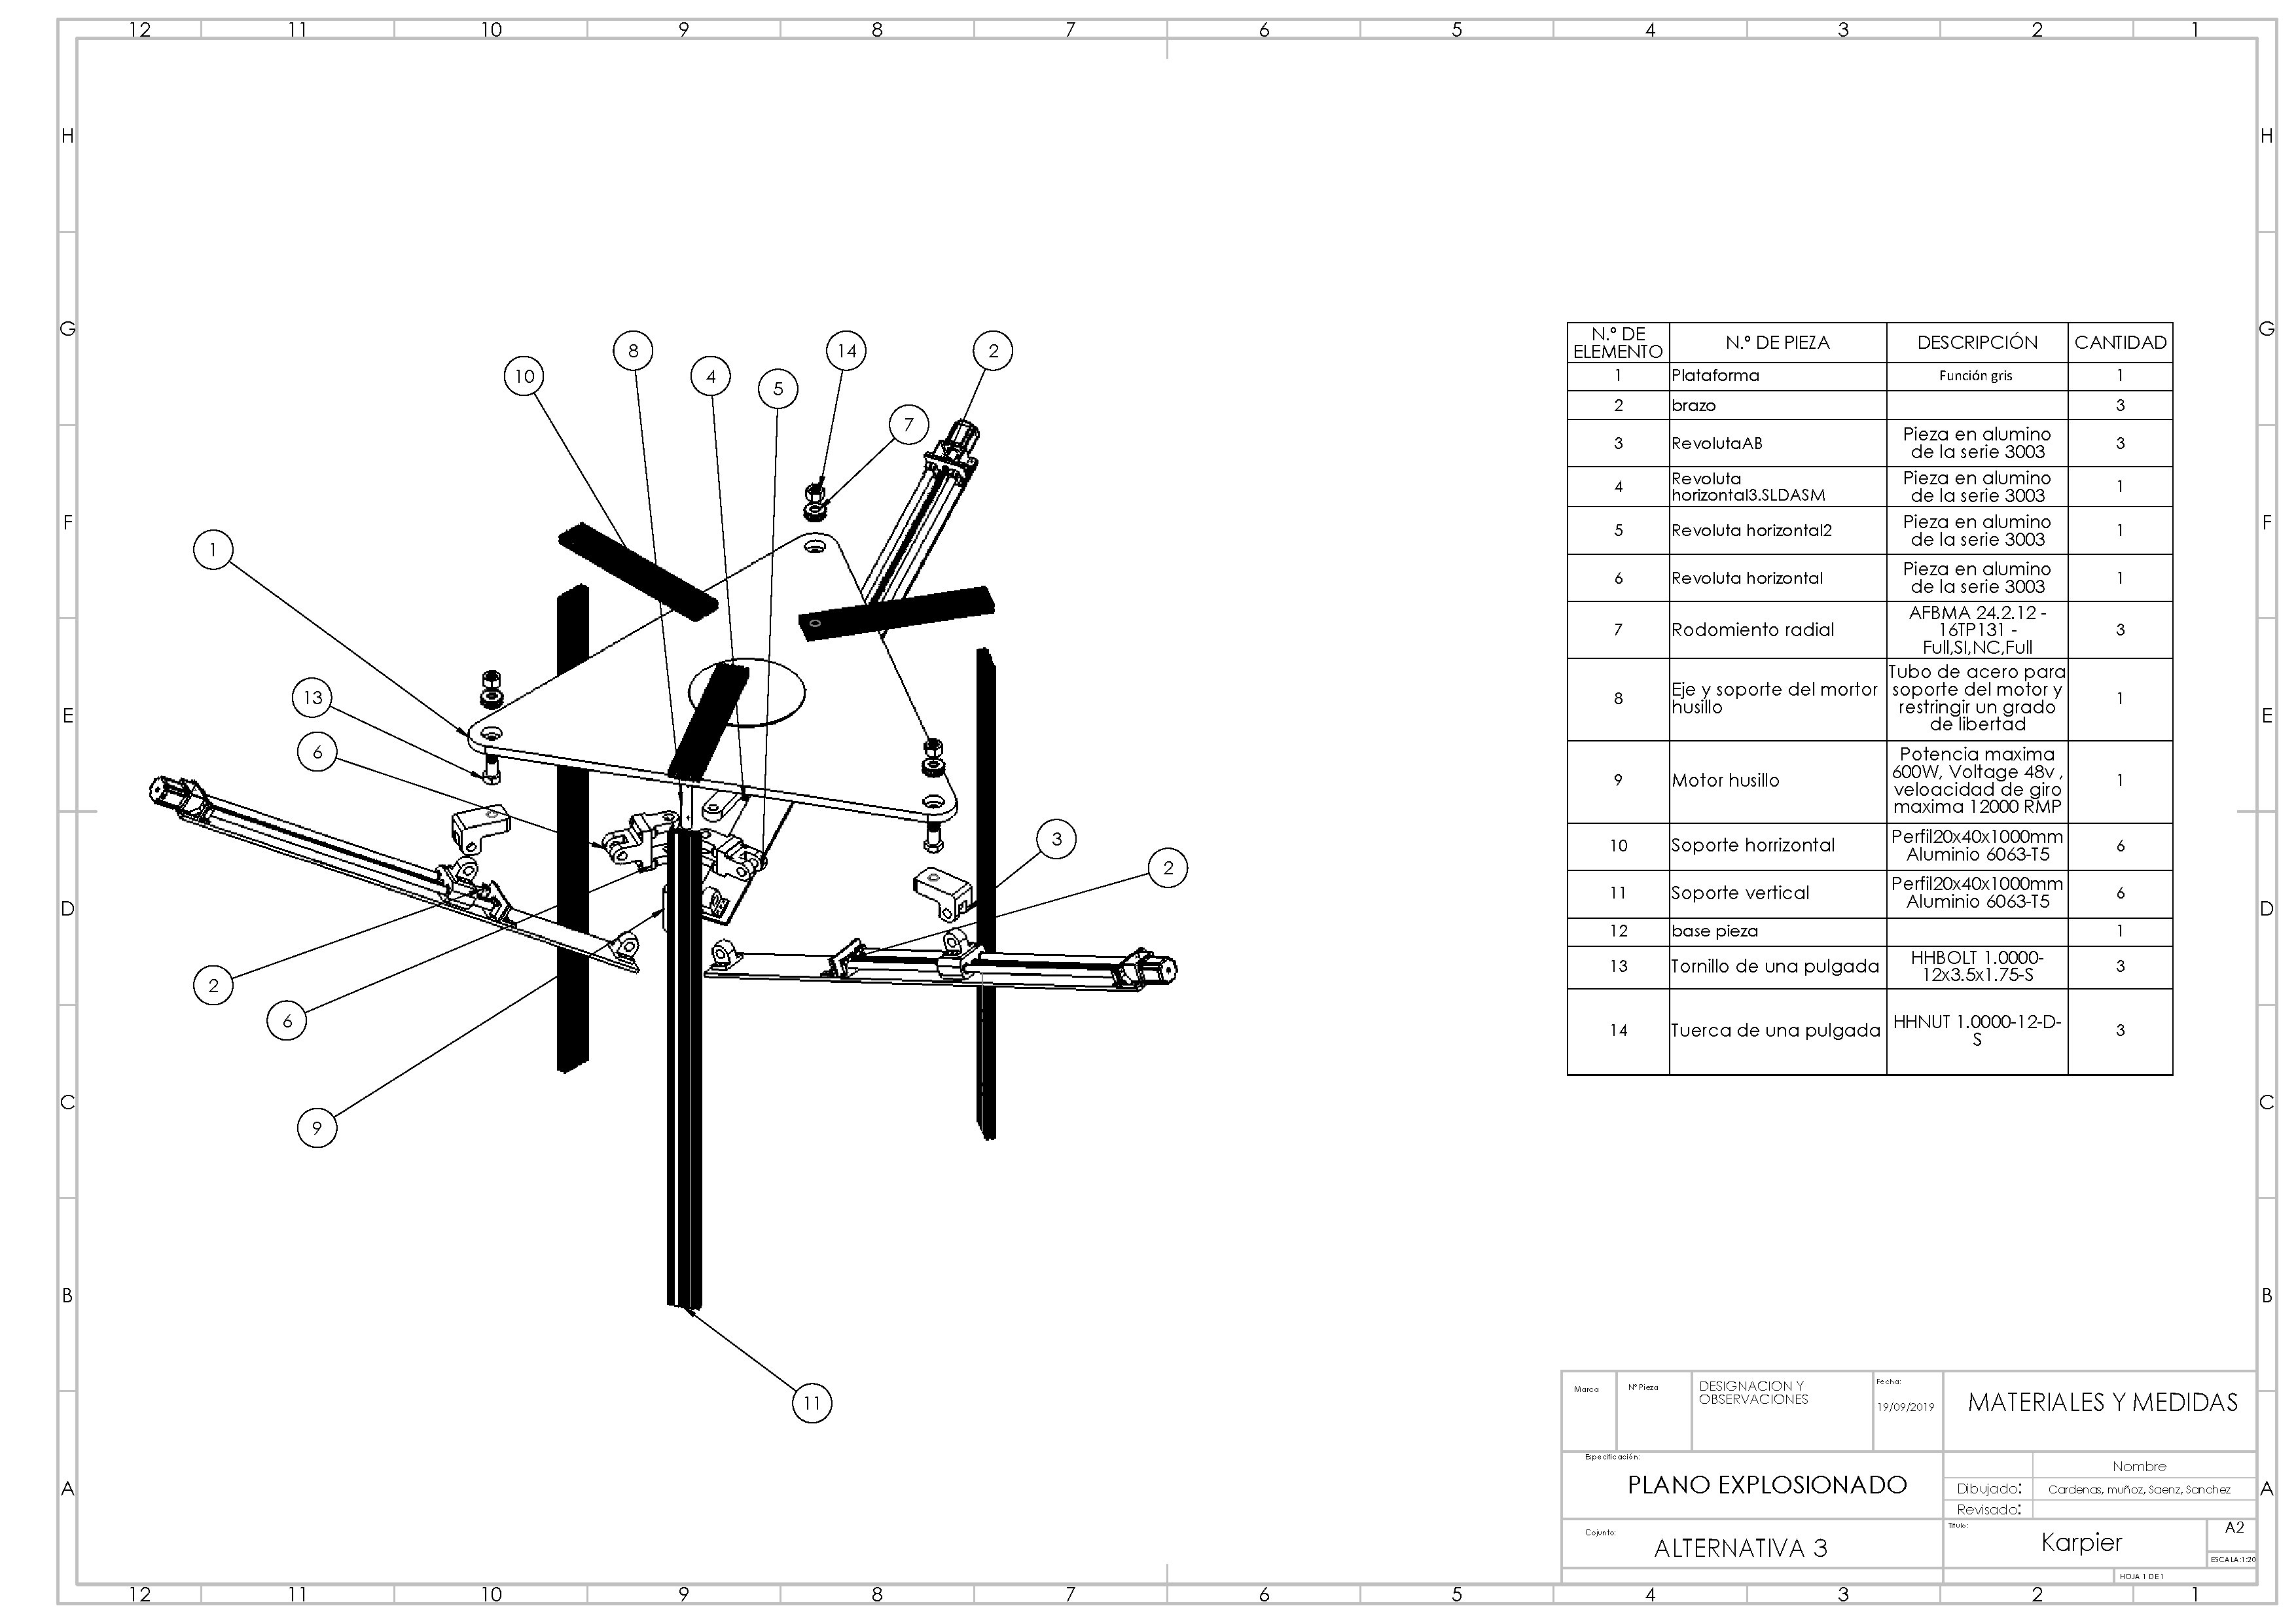
\includegraphics[width =  \textwidth]{Cap3_DisenoConceptual/Figura/Planowilliam.pdf}
    \caption{Lista de materiales, alternativa 3}{Fuente: Elaboración Propia}
    \label{fig:Plano_alt_3}
\end{figure}
\begin{figure}[ht]
    \centering
    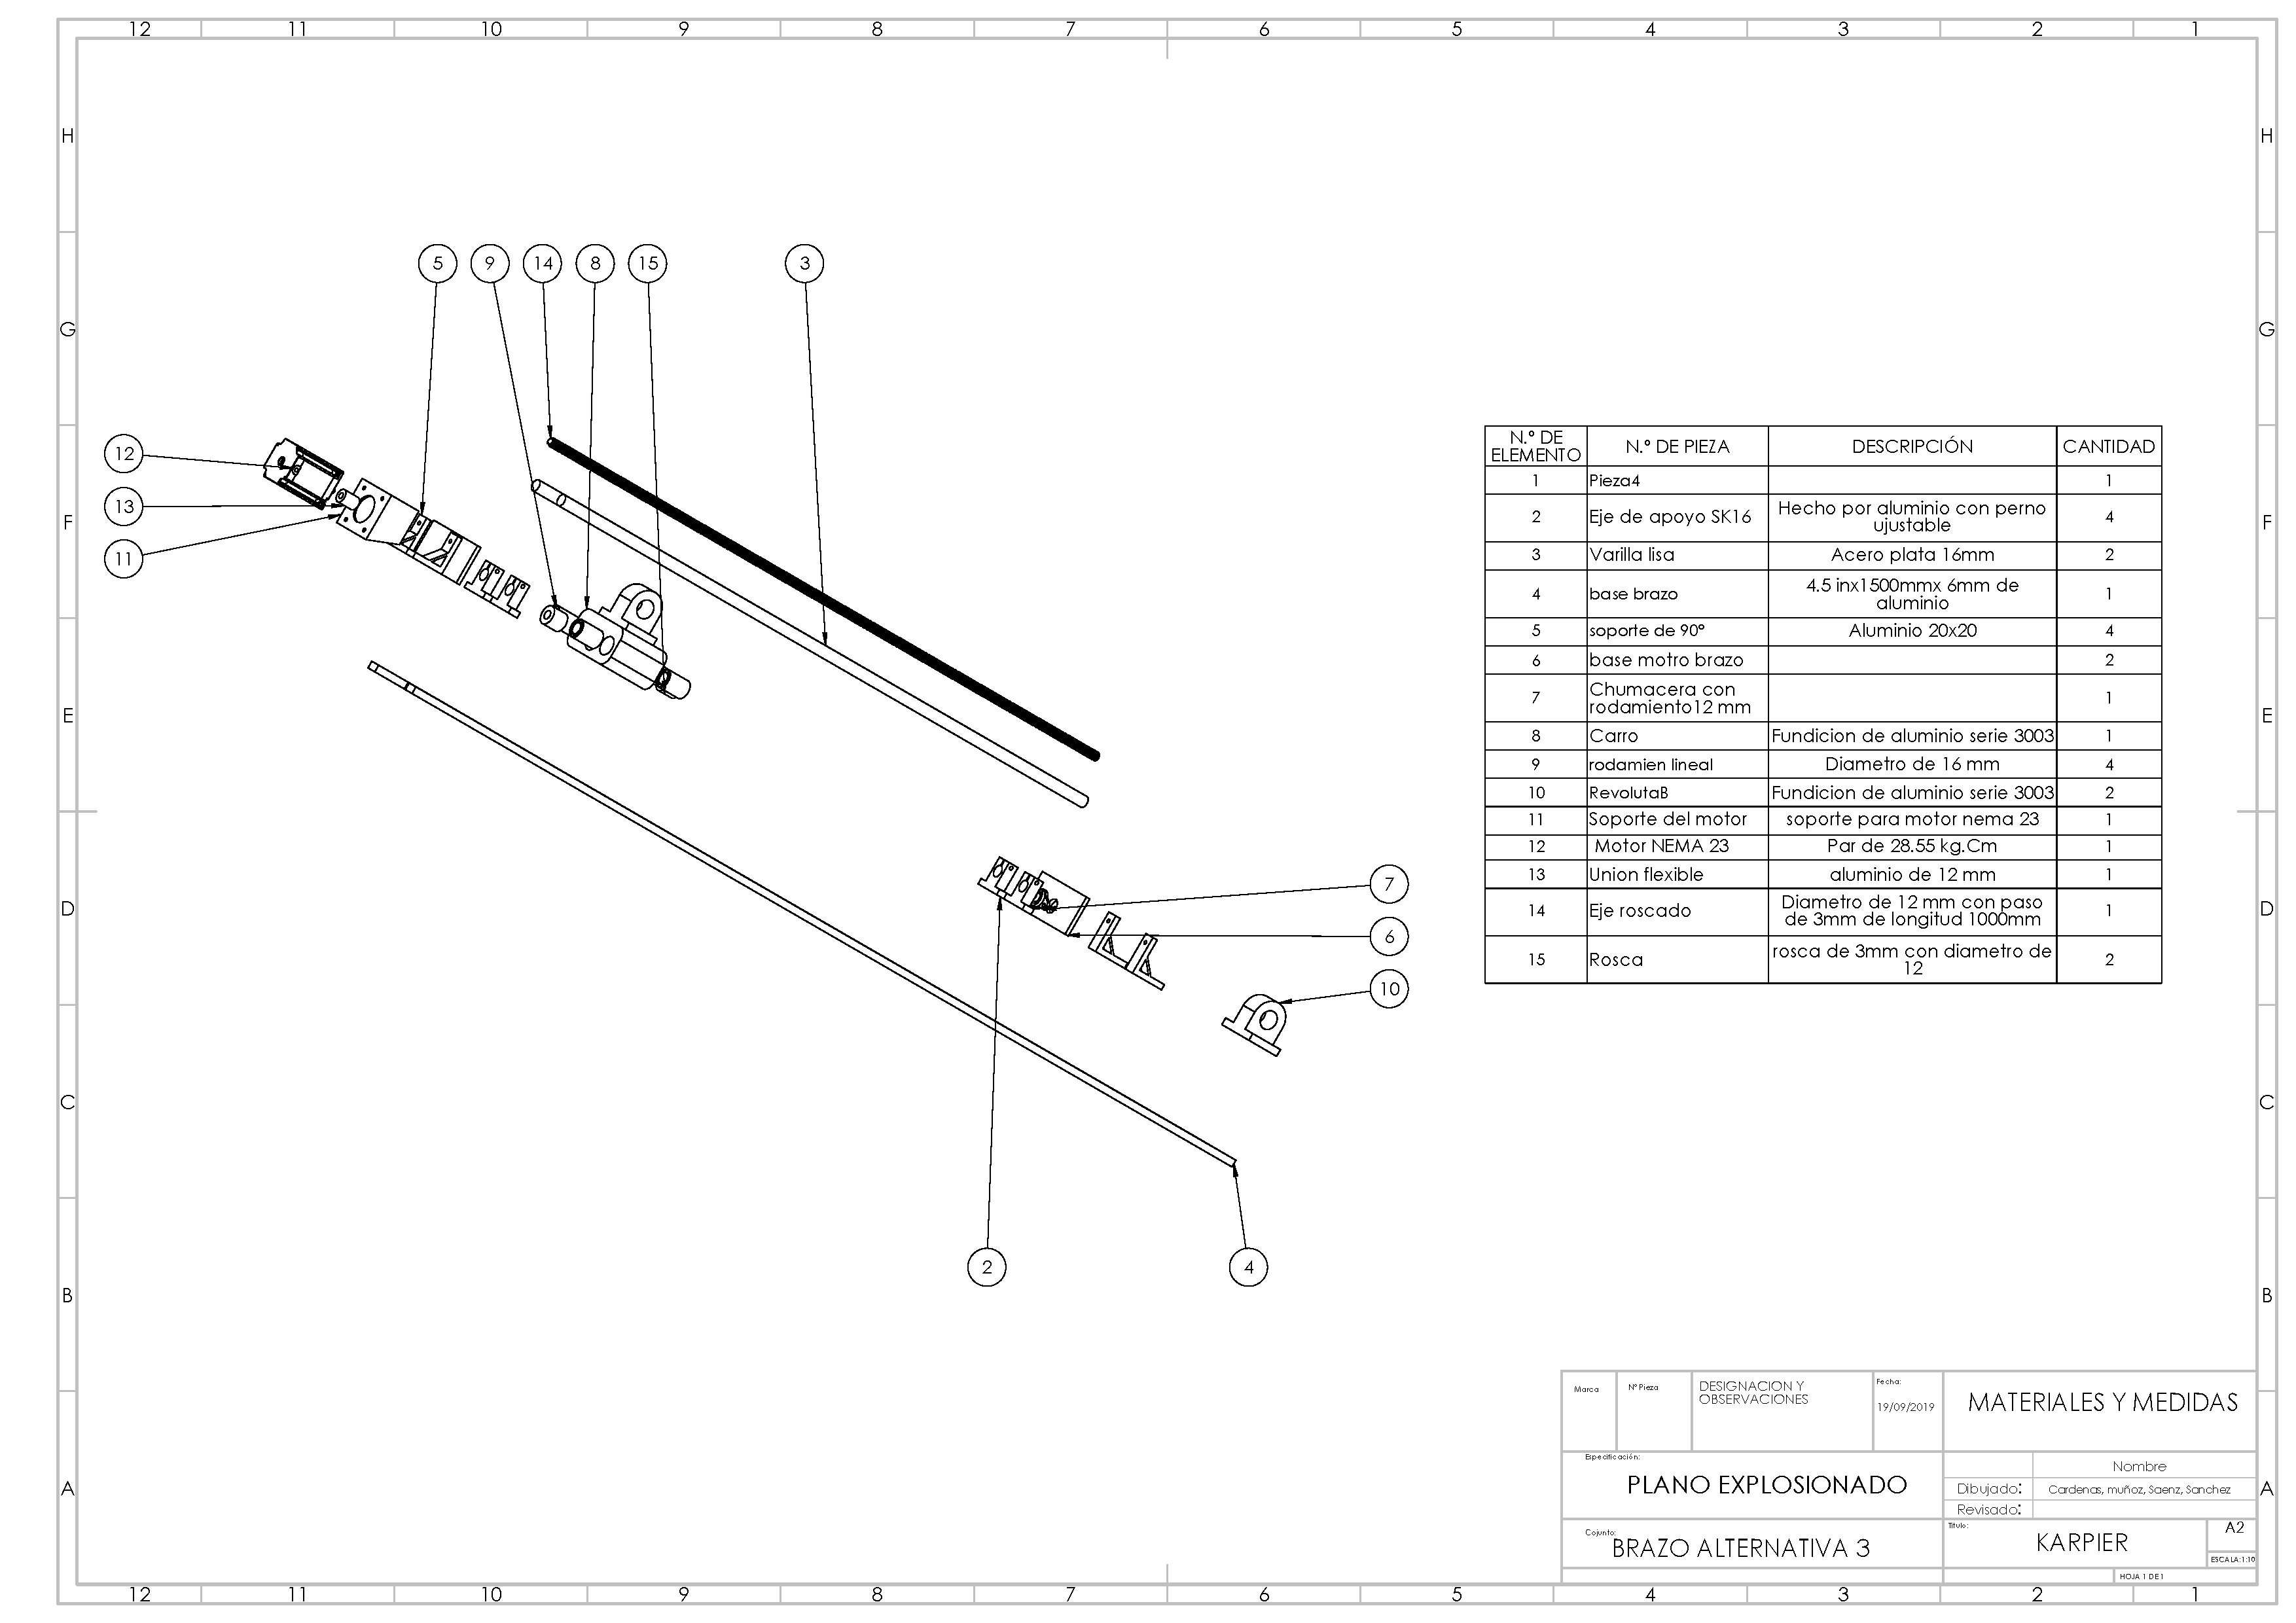
\includegraphics[width =  \textwidth]{Cap3_DisenoConceptual/Figura/PlanoBrazo.pdf}
    \caption{Lista de materiales Brazo, alternativa 3}{Fuente: Elaboración Propia}
    \label{fig:Plano_alt_3.2}
\end{figure}

\newpage
~
\newpage

\subsubsection{Presupuesto}
Una vez con el concepto de la alternativa establecido, se procedió a realizar un presupuesto para la posterior evaluación de viabilidad de la alternativa.
\begin{longtable}{| c | p{0.32\textwidth} | r | r | c | r |}
\hline \rowcolor[gray]{0.85}
 & Descripción & \multicolumn{1}{c|}{Valor Unitario} & \multicolumn{1}{c|}{Cantidad} & Unidades & \multicolumn{1}{c|}{Valor}  \\ \hline \endhead
\multirow{5}{*}{\rotatebox{90}{Diseño}}
 & Ingeniero de calculo & \$ 150.000,00 & 80,00 & horas & \$ 12.000.000,00 \\
 & Memorias y plano & \$ 15.000,00 & 40,00 & horas & \$ 600.000,00 \\
 & Software  & \$ 750.000,00 & 1,00 & - & \$ 750.000,00 \\ 
 & Interfaz & \$ 500.000,00 & 1,00 & - & \$ 500.000,00 \\
\cline{2-6} & \multicolumn{4}{c|}{ \textbf{Subtotal Diseño}} & \$ \textbf{13.850.000,00}  \\ \hline

% \multirow{18}{*}{\rotatebox{90}{Lista de Componentes}}
 & Motor Paso a Paso Nema 23 28.55 Kg.cm & \$ 225.676,00 & 3,00 & - & \$ 677.028,00 \\
 & Motor-Husillo 600W max,48 V max, 1200 Rpm max, DC & \$ 400.000,00 & 1,00 & - & \$ 400.000,00 \\
 & Tornillo de potencia 12 mm x 1 m & \$ 45.000,00 & 3,00 & - & \$ 135.000,00 \\
 & Acople Flexible D30L42 10 mm X 14 mm & \$ 35.890,00 & 3,00 & - & \$ 107.670,00 \\
 & Rosca Brida T8 - D 12 mm & \$ 36.904,86 & 3,00 & - & \$ 110.714,58 \\
 & Varilla de acero 16 mm x 0.5 m & \$ 68.300,00 & 6,00 & - & \$ 409.800,00 \\
 & Apoyo para varilla lisa de 16 mm & \$ 8.400,00 & 12,00 & - & \$ 100.800,00 \\
 & Lamina de aluminio de 4.5 pulg x 1/4 pulg x 1.5 m & \$ 25.000,00 & 3,00 & - & \$ 75.000,00 \\
 & Perfil de aluminio 20 mm x 40 mm x 1m & \$ 72.900,00 & 6,00 & - & \$ 437.400,00 \\
 & Perfil de aluminio 20 mm x 40 mm x 1.5m & \$ 90.200,00 & 6,00 & - & \$ 541.200,00 \\
 & Driver motor paso a paso Nema 23 & \$ 65.000,00 & 3,00 & - & \$ 195.000,00 \\
 & Revoluta Horizontal tipo 1 & \$ 15.000,00 & 1,00 & kg & \$ 15.000,00 \\
 & Revoluta Horizontal tipo 2 & \$ 15.000,00 & 6,24 & kg & \$ 93.600,00 \\
 & Revoluta Horizontal tipo 3 & \$ 15.000,00 & 3,47 & kg & \$ 52.000,00 \\
 & Carro Brazos & \$ 15.000,00 & 2,63 & kg & \$ 39.465,00 \\
 & Plataforma & \$ 50.000,00 & 16,98 & kg & \$ 849.060,00 \\
 & Rodamiento Lineal LM16UU & \$ 14.875,00 & 14,00 & - & \$ 208.250,00 \\
 & Chumacera K004 FL001 & \$ 12.300,00 & 3,00 & - & \$ 36.900,00 \\
 & Ordenador PC & \$ 3.600.000,00 & 1,00 & - & \$ 3.600.000,00 \\
 & Accesorios electricos & \$ 400.000,00 & 1,00 & - & \$ 400.000,00 \\
 & Tornilleria  & \$ 200.000,00 & 1,00 & - & \$ 200.000,00 \\
 & Sistema de limpieza & \$ 500.000,00 & 1,00 & - & \$ 500.000,00 \\
 & Sistema de refrigeración & \$ 500.000,00 & 1,00 & - & \$ 500.000,00 \\
 & Sistema de sujeccion & \$ 500.000,00 & 1,00 & - & \$ 500.000,00 \\
\cline{2-6}
\multirow{-18}{*}{\rotatebox{90}{Lista de Componentes}} & \multicolumn{4}{c|}{\textbf{Subtotal Lista de Componentes}} & \$ \textbf{10.183.887,58} \\ \hline

\multirow{4}{*}{\rotatebox{90}{Fabricación}}
 & Emsablador &  \$ 10.000,00  & 40,00 & horas &  \$ 400.000,00 \\
 & Ayudante  &  \$ 6.000,00  & 40,00 & horas &  \$ 240.000,00 \\
 & Surpervisor &  \$ 100.000,00  & 20,00 & horas &  \$ 2.000.000,00 \\
 \cline{2-6} & \multicolumn{4}{c|}{\textbf{Subtotal Fabricación}} & \$ \textbf{2.640.000,00} \\ \hline

\multirow{4}{*}{\rotatebox{90}{Equipos}} 
 & Pintura  &  \$ 20.000,00  & 4,00 & m2 &  \$ 80.000,00 \\
 & Herramientas &  \$ 350.000,00  & 1,00 & - &  \$ 350.000,00 \\
 & Centro de mecanizado  &  \$ 90.000,00  & 16,00 & horas &  \$ 1.440.000,00 \\
 \cline{2-6} & \multicolumn{4}{c|}{\textbf{Subtotal Sección}} & \$ \textbf{1.870.000,00} \\ \hline

\rowcolor[gray]{0.85} \multicolumn{5}{|c|}{\textbf{Subtotal}} & \$ \textbf{28.543.887,58} \\ \hline
\multicolumn{5}{|c|}{\textbf{Imprevistos (30\%)}} & \$ \textbf{8.563.166,27} \\ \hline
\rowcolor[gray]{0.85} \multicolumn{5}{|c|}{\textbf{Total}} & \$ \textbf{37.107.053,85} \\ \hline
\caption{Presupuesto de la Alternativa 3}{Fuente: Elaboración Propia}
\end{longtable}

\section{Proceso Analítico de Jerarquía  (AHP)}
%\subsection{Matrices de Comparación por Pares}
\begin{longtable}{|>{\columncolor[gray]{0.85}}c|c|c|c|c|c|c|c|}
\multicolumn{8}{c}{\textbf{COSTO DE ADQUISICION}} \\ \hline
\rowcolor[gray]{0.85} & Alternativa 1 & Alternativa 2 & Alternativa 3 & \multicolumn{3}{c}{Matriz Normalizada} & Promedio \\ \hline
Alternativa 1 & 1 & 0.2 & 0.3333 & 0,1111 & 0,1304 & 0,0769 & 0.1061 \\ \hline
Alternativa 2 & 5 & 1 & 3 & 0,5555 & 0,6521 & 0,6923 & 0.6333 \\ \hline
Alternativa 3 & 3 & 0.3333 & 1 & 0,33 & 0,2173 & 0,2307 & 0.2604 \\ \hline
Total & 9 & 1.53 & 4.33\\ \cline{1-4}
\caption{Ponderación del Costo de Adquisición}{Fuente: Elaboración Propia}
\end{longtable}
\begin{longtable}{|>{\columncolor[gray]{0.85}}c|c|c|c|c|c|c|c|}
\multicolumn{8}{c}{\textbf{COSTO DE MANTENIMIENTO}} \\ \hline
\rowcolor[gray]{0.85} & Alternativa 1 & Alternativa 2 & Alternativa 3 & \multicolumn{3}{c}{Matriz Normalizada} & Promedio \\ \hline
Alternativa 1 & 1 & 5 & 3 & 0,6521 & 0.5556 & 0,6923 & 0.6333 \\ \hline
Alternativa 2 & 0.2 & 1 & 0.3333 & 0,1304 & 0,1111 & 0,0769 & 0.1061 \\ \hline
Alternativa 3 & 0.3333 & 3 & 1 & 0.2173 & 0,33 & 0,2307 & 0.2604 \\ \hline
Total & 9 & 1.53 & 4.33\\ \cline{1-4}
\caption{Ponderación del Costo de Mantenimiento}{Fuente: Elaboración Propia}
\end{longtable}
%\newpage
\begin{longtable}{|>{\columncolor[gray]{0.85}}c|c|c|c|c|c|c|c|}
\multicolumn{8}{c}{\textbf{COSTO DE OPERATIVO}} \\ \hline
\rowcolor[gray]{0.85} & Alternativa 1 & Alternativa 2 & Alternativa 3 & \multicolumn{3}{c}{Matriz Normalizada} & Promedio \\ \hline
Alternativa 1 & 1 & 0.2 & 0.1428  & 0,0769 & 0.0322 & 0,1063 & 0.0718 \\ \hline
Alternativa 2 & 5 & 1 & 0.2 & 0,3846 & 0,1612 & 0,1489 & 0.2316 \\ \hline
Alternativa 3 & 7 & 5 & 1 & 0.5384 & 0,8064 & 0,7446 & 0.6965 \\ \hline
Total & 13 & 6.2 & 1.3428 \\ \cline{1-4}
\caption{Ponderación del Costo de Operativo}{Fuente: Elaboración Propia}
\end{longtable}
\input{Cap3_DisenoConceptual/Tablas/Precisión.tex}
\begin{longtable}{|>{\columncolor[gray]{0.85}}c|c|c|c|c|c|c|c|}
\multicolumn{8}{c}{\textbf{COMPACIDAD}} \\ \hline
\rowcolor[gray]{0.85} & Alternativa 1 & Alternativa 2 & Alternativa 3 & \multicolumn{3}{c}{Matriz Normalizada} & Promedio \\ \hline
Alternativa 1 & 1 & 5 & 3 & 0,6521 & 0,5555 & 0,6920 & 0.6333 \\ \hline
Alternativa 2 & 0.2 & 1 & 0.3333 & 0,1304 & 0,1111 & 0,0769 & 0.1061 \\ \hline
Alternativa 3 & 0.3333 & 0.3 & 1 & 0,2127 & 0,3333 & 0,2307 & 0.2604 \\ \hline
Total & 1.5333 & 9 & 4.3333\\ \cline{1-4}
\caption{Ponderación de la Compacidad}{Fuente: Elaboración Propia}
\end{longtable}
\begin{longtable}{|>{\columncolor[gray]{0.85}}c|c|c|c|c|c|c|c|}
\multicolumn{8}{c}{\textbf{RECONFIGURABILIDAD}} \\ \hline
\rowcolor[gray]{0.85} & Alternativa 1 & Alternativa 2 & Alternativa 3 & \multicolumn{3}{c}{Matriz Normalizada} & Promedio \\ \hline
Alternativa 1 & 1 & 5 & 3 & 0,6521 & 0.5555 & 0,6923 & 0.6333 \\ \hline
Alternativa 2 & 0.2 & 1 & 0.3333 & 0,1304 & 0,1111 & 0,0769 & 0.1061 \\ \hline
Alternativa 3 & 0.3333 & 3 & 1 & 0.2173 & 0,3333 & 0,2307 & 0.2604\\ \hline
Total & 1.5333 & 9 & 4.3333\\ \cline{1-4}
\caption{Ponderación de la Reconfigurabilidad}{Fuente: Elaboración Propia}
\end{longtable}
%\newpage
\begin{longtable}{|>{\columncolor[gray]{0.85}}c|c|c|c|c|c|c|c|}
\multicolumn{8}{c}{\textbf{SEGURIDAD}} \\ \hline
\rowcolor[gray]{0.85} & Alternativa 1 & Alternativa 2 & Alternativa 3 & \multicolumn{3}{c}{Matriz Normalizada} & Promedio \\ \hline
Alternativa 1 & 1 & 5 & 3 & 0,6521 & 0.5555 & 0,6923 & 0.6333 \\ \hline
Alternativa 2 & 0.2 & 1 & 0.3333 & 0,1304 & 0,1111 & 0,0769 & 0.1061 \\ \hline
Alternativa 3 & 0.3333 & 3 & 1 & 0.2173 & 0,3333 & 0,2307 & 0.2604\\ \hline
Total & 1.5333 & 9 & 4.3333\\ \cline{1-4}
\caption{Ponderación de la Seguridad}{Fuente: Elaboración Propia}
\end{longtable}
\begin{longtable}{|>{\columncolor[gray]{0.85}}c|c|c|c|c|c|c|c|}
\multicolumn{8}{c}{\textbf{SISTEMA DE CONTROL}} \\ \hline
\rowcolor[gray]{0.85} & Alternativa 1 & Alternativa 2 & Alternativa 3 & \multicolumn{3}{c}{Matriz Normalizada} & Promedio \\ \hline
Alternativa 1 & 1 & 0.2 & 0.25 & 0,1 & 0.1304 & 0,0588 & 0.0964 \\ \hline
Alternativa 2 & 5 & 1 & 3 & 0,5 & 0,6521 & 0,7058 & 0.6093 \\ \hline
Alternativa 3 & 4 & 0.3333 & 1 & 0.4 & 0,2173 & 0,2352 & 0.2842\\ \hline
Total & 10 & 1.5333 & 4.25\\ \cline{1-4}
\caption{Ponderación del Sistema de Control}{Fuente: Elaboración Propia}
\end{longtable}
\begin{longtable}{|>{\columncolor[gray]{0.85}}c|c|c|c|c|c|c|c|}
\multicolumn{8}{c}{\textbf{CAPACIDAD DE CARGA}} \\ \hline
\rowcolor[gray]{0.85} & Alternativa 1 & Alternativa 2 & Alternativa 3 & \multicolumn{3}{c}{Matriz Normalizada} & Promedio \\ \hline
Alternativa 1 & 1 & 0.2 & 0.1428 & 0,0769 & 0.0476 & 0,0967 & 0.0737 \\ \hline
Alternativa 2 & 5 & 1 & 0.3333 & 0,3846 & 0,2380 & 0,2258 & 0.2828 \\ \hline
Alternativa 3 & 7 & 3 & 1 & 0.5348 & 0,7142 & 0,6774 & 0.6433\\ \hline
Total & 13 & 4.2 & 1.4761\\ \cline{1-4}
\caption{Ponderación de la Capacidad de Carga}{Fuente: Elaboración Propia}
\end{longtable}
%\newpage

%\subsection{Matriz de selección de Alternativas}
\input{Cap3_DisenoConceptual/Tablas/Matrizdedecisión.tex}
%\newpage
\begin{landscape}
    \begin{table}
\centering
\footnotesize
\begin{tabular}{|>{\columncolor[gray]{0.85}}c|c|c|c|c|c|c|c|c|c|c|c|c|c|c|}
%\rowcolor[gray]{0.85} \hline
\multicolumn{14}{c}{\textbf{\uppercase{Analisis de sensibilidad para alternativas}}}\\ \hline
\rowcolor[gray]{0.85}
\textbf{Criterios} & \rotatebox{90}{Costo de Adquisicion} & \rotatebox{90}{Costo de Mantenimiento} & \rotatebox{90}{Costo operativo} & \rotatebox{90}{Precision / Rigidez} & \rotatebox{90}{Seguridad} & \rotatebox{90}{Compacidad} & \rotatebox{90}{Reconfigurabilidad} & \rotatebox{90}{Control} & \rotatebox{90}{Capacidad de Carga} & \rotatebox{90}{Total} & \rotatebox{90}{Ponderación 1} & \rotatebox{90}{Ponderación 2} & \rotatebox{90}{Ponderación 3} \\ \hline
Alternativa 1 & 0.1062 & 0.6333 & 0.0719 & 0.1149 & 0.6333 & 0.6333 & 0.0738 & 0.0964 & 0.0738 & 0.246 & 0.235 & 0.332 & 0.145 \\ \hline
Alternativa 2 & 0.6333& 0.1062 & 0.2316 & 0.1822 & 0.1062 & 0.1062 & 0.6434 & 0.6194 & 0.2828 & 0.321 & 0.328 & 0.292 & 0.4 \\ \hline
Alternativa 3 & 0.2605 & 0.2605 & 0.6965  & 0.7028 & 0.2605 & 0.2605 & 0.2828 & 0.2842 & 0.6434 & 0.432 & 0.437 & 0.376 & 0.455\\ \hline
Ponderación & 0.1652 & 0.0346 & 0.702  & 0.2548 & 0.2257 & 0.0144 & 0.0287 & 0.1427 & 0.0619\\ \cline{1-10}
Total & 0.1652 & 0.0346 & 0.072 & 0.2548 & 0.2257 & 0.0144 & 0.0287 & 0.1427 & 0.0619\\ \cline{1-10}
Ponderación 1 & 0.1952 & 0.054 & 0.1420  & 0.1548 & 0.1211 & 0.0856 & 0.0313 & 0.1027 & 0.1119\\ \cline{1-10}
Ponderación 2 & 0.0652 & 0.0246 & 0.0520  & 0.0848 & 0.1746 & 0.2456 & 0.0687 & 0.1527 & 0.1319\\ \cline{1-10}

Ponderación 3 & 0.2252 & 0.0354 & 0.1020  & 0.3148 & 0.0348 & 0.0144 & 0.0887 & 0.1727 & 0.0119\\ \cline{1-10}


\end{tabular}
\caption{Analisis de sensibilidad para alternativas}{Fuente: Elaboración Propia}
\label{table:SensibilityAnalysis}
\end{table}
\end{landscape}

\section{Alternativa Escogida}
\begin{figure}[hbt!]
    \centering
    \begin{subfigure}{0.5\textwidth}
        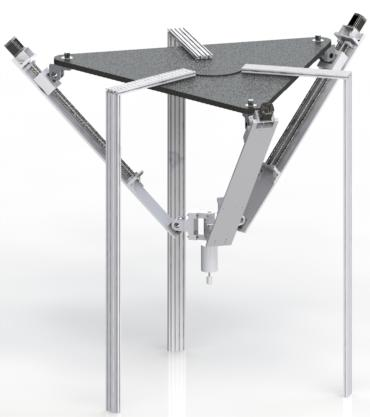
\includegraphics[width = \linewidth]{Cap3_DisenoConceptual/Figura/Solucion1.JPG}
        \caption{Sistema Completo}
    \end{subfigure}
    \begin{subfigure}{0.5\textwidth}
        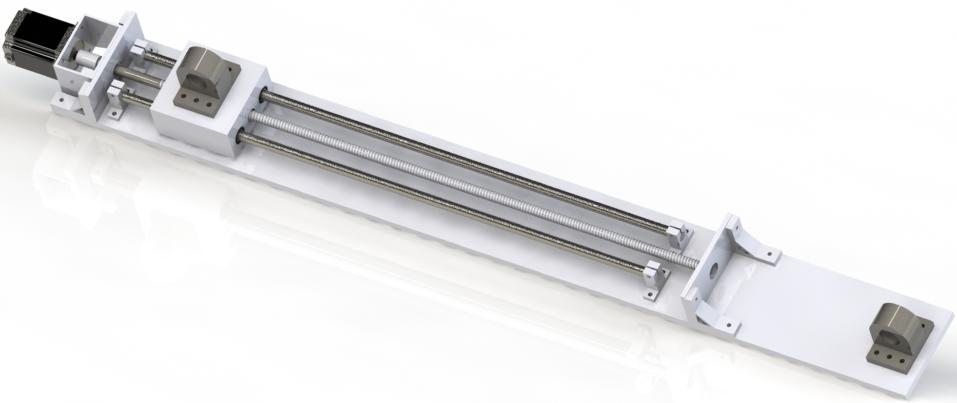
\includegraphics[width = \linewidth]{Cap3_DisenoConceptual/Figura/Solucion2.JPG}
        \caption{Brazo Completo}
    \end{subfigure}
    \caption{Renderizado de la Alternativa Escogida}
    \label{fig:RenderSolucion}
\end{figure}
